\documentclass{itkmitlcoop}

\usepackage{afterpage}
\usepackage{graphicx,amsmath,latexsym,amssymb,amsthm}
\usepackage{indentfirst}
\usepackage{cite}
\usepackage[final]{pdfpages}

% ##### Code Snippets Setting https://www.overleaf.com/learn/latex/Code_listing
\usepackage{listings}
\usepackage{xcolor}
\usepackage{lstfiracode}
 \setmonofont{Fira Code}[
 Contextuals=Alternate  % Activate the calt feature
 ]
\definecolor{codegreen}{rgb}{0,0.6,0}
\definecolor{codegray}{rgb}{0.5,0.5,0.5}
\definecolor{codepurple}{rgb}{0.58,0,0.82}
\definecolor{backcolour}{rgb}{0.95,0.95,0.92}

\lstset{style=FiraCodeStyle,
	basicstyle=\ttfamily\footnotesize,,
		backgroundcolor=\color{backcolour},   
	commentstyle=\color{codegreen},
	keywordstyle=\color{magenta},
	numberstyle=\tiny\color{codegray},
	stringstyle=\color{codepurple},
	breakatwhitespace=false,         
	breaklines=true,                 
	captionpos=b,                    
	keepspaces=true,                 
	numbers=left,                    
	numbersep=5pt,                  
	showspaces=false,                
	showstringspaces=false,
	showtabs=false,                  
	tabsize=2,
	escapeinside={<@}{@>},
}


% ##### Set indent after new line on bibliography
\def\bibindent{2.1em}
\makeatletter
\let\old@biblabel\@biblabel
\def\@biblabel#1{\old@biblabel{#1}\kern\bibindent}
\let\old@bibitem\bibitem
\def\bibitem#1{\old@bibitem{#1}\leavevmode\kern-\bibindent}
\makeatother

\graphicspath{ {images/} }

%Your thesis title (THAI)
\newcommand{\ThesisTiTle}{การศึกษาการประเมินช่องโหว่ความปลอดภัยของเว็บแอปพลิเคชันในกรณีศึกษาที่ได้จากการฝึกงานสหกิจ ณ บริษัท เซค คอนซัลท์ (ไทยแลนด์) จำกัด}
%Your thesis title (ENG)
\newcommand{\ThesisTiTleENG}{A STUDY ON PENETRATION TESTING OF WEB APPLICATIONS: CASE STUDIES FROM CO-OPERATIVE EDUCATION AT SEC CONSULT (THAILAND) CO., LTD.}
\newcommand{\ThesisTiTleENGSnakecase}{A Study on Penetration Testing of Web Applications: Case Studies from Co-Operative Education at SEC Consult (Thailand) Co., Ltd}
%Your name
\newcommand{\AuName}{นายวีรภัทร ทรัพย์สมบูรณ์}
%Your name ENG
\newcommand{\AuNameENG}{WEERUHPUTT SUPSOHMBOON}
\newcommand{\AuNameENGSnakecase}{Weeruhputt Supsohmboon}
%Your student ID
\newcommand{\SId}{59070162}
%Your advisor
\newcommand{\Advisor}{ผู้ช่วยศาสตราจารย์ ดร. สุเมธ ประภาวัต}
%Your advisor english
\newcommand{\AdvisorEng}{Assistance Professor Dr. Sumet Prabhavat}
%Your advisor employee
\newcommand{\Exami}{นายชาญณรงค์ ตัณฑวนันท์}
%สถานประกอบการ
\newcommand{\Company}{บริษัท เซค คอนซัลท์ (ไทยแลนด์) จำกัด}
\newcommand{\CompanyEng}{SEC Consult (Thailand) Co., Ltd.}
%ภาคเรียนที่ (in normal letters)
\newcommand{\Sem}{1}
%ปีการศึกษา (in normal letters)
\newcommand{\AcaY}{2562}
%ปีการศึกษา (in normal letters)
\newcommand{\AcaYAD}{2019}
%วันส่งรายงาน
\newcommand{\SubD}{15 พฤษจิกายน พ.ศ. 2562}
%วันเริ่มทำงาน
\newcommand{\StartDWork}{3 มิถุนายน พ.ศ. 2562}
%วันสุดท้ายของการทำงาน
\newcommand{\EndDWork}{29 พฤษจิกายน พ.ศ. 2562}
%ที่อยู่สถานประกอบการ
\newcommand{\Address}{29/1 ปิยะเพลส หลังสวน ชั้น 16 ห้อง 16บี ซอยหลังสวน ถนนเพลินจิต แขวงลุมพินี \newline เขตปทุมวัน กรุงเทพ 10330}
%เว็บไซต์สถานประกอบการ
\newcommand{\Website}{https://sec-consult.com/en/}
%ตำแหน่งานที่ปฏิบัติ
\newcommand{\Position}{ผู้ช่วยผู้ให้คำปรึกษาด้านความปลอดภัย}

\begin{document}    
    \frontmatter
    \pagenumbering{Roman}
    \lhead{}\rhead{}\chead{}\lfoot{}\cfoot{\thepage}\rfoot{}
    
    \makecover
    \makeinnercover
    \makeengcover
    \makecopyrightcover
    \makeletter
    \makeack{
        \begin{enumerate}
            \item \Exami \quad ตำแหน่ง Security Consultant
            %\item นายธนภณ ซู \quad ตำแหน่ง Security Consultant
        \end{enumerate}
    }
    \makeapproveletter
    
    % Setting margin for page numbering on frontmatter
    \newgeometry{top=1in, bottom=1in, left=1.5in, right=1in, includefoot}
    
   \makeabstract{
    		รายงานการปฏิบัติงานสหกิจศึกษาฉบับนี้กล่าวถึงขั้นตอนการทำงานเจาะระบบ และรายการช่องโหว่ซึ่งจัดหมวดหมู่ตาม OWASP Top 10 และรวบรวมมาจากการฝึกงานสหกิจศึกษา ณ \Company ซึ่งเป็นบริษัทที่ดำเนินธุรกิจให้คำปรึกษาด้านความปลอดภัยของระบบสารสนเทศทั้งในองค์กร และผลิตภัณฑ์สาธารณะที่บุคคลทั่วไปใช้งาน
    		
    		งานที่ผู้เขียนได้ฝึกงานสหกิจศึกษาเป็นงานค้นหาช่องโหว่ในระบบสารสนเทศของลูกค้า พร้อมทั้งรายงานช่องโหว่ที่พบเจอและวิธีการแก้ไขช่องโหว่ให้กับลูกค้า ซึ่งใช้การบูรณาการทางด้าน Software Engineer และ Computer Network เข้ามาคาดเดากระบวนการทำงานของระบบ เพื่อช่วยให้ค้นหาช่องโหว่ได้ง่ายขึ้น
    		
    		โดยส่วนมากช่องโหว่ที่พบเจอมักจะไม่รุนแรงมากนัก กล่าวคือเพียงแค่ขาดการตั้งค่าที่ส่งเสริมความปลอดภัยให้ดีขึ้น แต่ทว่าก็พบเจอช่องโหว่ร้ายแรงบ้างเหมือนกัน ซึ่งช่องโหว่ที่ร้ายแรงมากที่สุดที่เคยพบเจอคือช่องโหว่ที่สามารถส่งคำสั่งไปทำงานบน Server ได้ ทำให้สามารถเข้าถึงการตั้งค่าและข้อมูลต่าง ๆ ของระบบได้
    }

    \makeengabstract{
		This cooperative internship report describes the penetration testing process and the vulnerability collection, which is categorized according to the OWASP Top 10 and gathered from a cooperative internship at \CompanyEng, a company that provides information security consulting services for many organizations.
		
		The work that the author has practiced in cooperative studies is to search for security vulnerabilities in the customer information system. Including reporting vulnerabilities and resolving vulnerabilities for customers, which uses the integration of software engineers and computer networks skills to predict system processes to help find vulnerabilities more efficiently.
		
		In most cases, the founded vulnerabilities are not entirely critical. Many of them are just lack of settings that increase security, e.g., HTTP Security Headers. But the most severe vulnerability which had been found was the ability to send commands to run on the server, allowing access to system settings and data.
		
    }

    \newpage
    \addcontentsline{toc}{chapter}{สารบัญ}
    \tableofcontents
    
    %\newpage
    %\addcontentsline{toc}{chapter}{สารบัญตาราง}
    %\listoftables
    
    \newpage
    \addcontentsline{toc}{chapter}{สารบัญรูป}
    \listoffigures
    
    % Reset frontmatter page numbering margin, back to original margin from class file
    \restoregeometry

    \mainmatter
    \lhead{}\rhead{\thepage}\chead{}\lfoot{}\cfoot{}\rfoot{}
    
    \chapter{บทนำ}
\label{chapter:introduction}

\section{ที่มาและความสำคัญ}

ในช่วงสองถึงสามปีที่ผ่านมา ข่าวด้านความปลอดภัยทางคอมพิวเตอร์ได้เกิดขึ้นบ่อยครั้ง ไม่ว่าจะเป็นข่าวที่เกิดขึ้นกับบุคคลธรรมดาสามัญ ที่มีผู้ที่ไม่หวังดีขโมยรหัสผ่าน Facebook ผ่านช่องทางหลอกลวง เช่น หลอกให้ผู้ใช้งาน Facebook ตอบกระทู้ด้วยรหัสผ่านบัญชีผู้ใช้ของตัวเอง เพื่อสุ่มแจกของรางวัล ทั้งที่จริง ๆ แล้วเป็นการหลอกลวง และได้นำรหัสผ่านนั้นไปใช้ปลอมตัวเป็นเจ้าของบัญชี เพื่อที่จะไปหลอกยืมเงินผู้อื่น ซึ่งทำให้เจ้าของบัญชีที่แท้จริงนั้นสูญเสียความน่าเชื่อถือ และเกิดความเข้าใจผิดขึ้น หรือแม้แต่บริษัทการสื่อสารแห่งหนึ่งที่ดูน่าเชื่อถือก็สามารถละเลยเรื่องความปลอดภัยของระบบจนทำให้ข้อมูลรูปสำเนาบัตรประชาชนเปิดเผยบนอินเตอร์เน็ตโดยที่ไม่มีการป้องกันใด ๆ ซึ่งอาจจะมีผู้ที่ไม่หวังดีนำข้อมูลไปใช้ปลอมแปลงเอกสารได้ ท้ายที่สุดมีผู้ประสงค์ดีได้รายงานไปยังบริษัท แต่ก็ต้องใช้เวลาถึงหนึ่งเดือนในการแก้ไขตั้งค่าข้อมูลไม่ให้สาธารณะเข้าถึงได้ \cite{truemoveh}

จะเห็นว่าภัยอันตรายทางคอมพิวเตอร์สามารถประสบพบเจอกับตัว ได้ทั้งทางตรงและทางอ้อม กล่าวคือถ้าเราไม่หลงกลเปิดแผยรหัสผ่านส่วนตัวให้กับผู้อื่น ก็อาจจะมีบริษัทที่เราเป็นลูกค้าทำข้อมูลส่วนตัวเราหลุดรอดออกมาสู่โลกอินเตอร์เน็ตด้วยความผิดพลาด ดังนั้นการที่เรามีความรู้ติดตัวด้านความปลอดภัยของคอมพิวเตอร์ไว้ก็จะช่วยลดความเสี่ยงที่จะเกิดผลกระทบทางตรงได้ เช่น ตั้งรหัสผ่านแต่ละบัญชีไม่ซ้ำกันและไม่ใช้วันเกิดหรือข้อมูลส่วนตัวเป็นส่วนประกอบของรหัสผ่าน เพื่อให้ยากต่อการเดาของผู้ไม่หวังดี  รู้จักวิธีแยกแยะจดหมายอิเล็กทรอนิกส์ที่เป็นประเภทหลอกลวง หรือแอบแฝงโปรแกรมที่ไม่หวังดี ซึ่งองค์ความรู้เหล่านี้สามารถหาได้ตามอินเทอร์เน็ต ส่วนวิธีการลดความเสี่ยงที่จะเกิดผลกระทบทางอ้อมกับตัวเรานั้นองค์กรหรือหน่วยงานรัฐและเอกชนจะต้องหมั่นตรวจสอบและดูแลรักษาความปลอดภัยระบบสารสนเทศของตัวเองไม่ให้มีช่องโหว่ และหมั่นค้นคว้าข่าวสารด้านความปลอดภัยและนำมาปรับปรุงให้กับระบบของตัวเองอยู่เสมอ 

ซึ่งงานของผู้เขียนนั้นเป็นงานค้นหาช่องโหว่ในระบบสารสนเทศของลูกค้า ทั้งใช้งานภายในและสาธารณะที่มีผู้ใช้งานจำนวนมาก

ในรายงานนี้มีจุดมุ่งหมายเพื่อรวบรวมช่องโหว่บน Web Platform ที่พบจอบ่อย ๆ จากการปฏิบัติงานและนำมาจัดทำรายงาน โดยจัดเป็นหมวดหมู่ตาม OWASP Top 10 เพื่อให้ผู้ดูแลหรือผู้พัฒนาระบบเทคโนโลยีสารสนเทศในหน่วยงานหรือองค์กรต่าง ๆ และผู้เริ่มต้นศึกษาด้านความปลอดภัยของคอมพิวเตอร์ศึกษาข้อมูลเป็นกรณีศึกษา และนำไปปรับใช้ ปรับปรุง และแก้ไขระบบในหน่วยงานตนเอง

\newpage
\section{วัตถุประสงค์ของการปฏิบัติงาน}
\begin{enumerate}
	\item เพื่อให้ผู้ดูแลหรือพัฒนาระบบในหน่วยงานหรือองค์กรต่าง ๆ ได้นำวิธีการตรวจสอบช่องโหว่จากรายงานฉบับนี้ไปปรับปรุงแก้ไขระบบของตน
	\item เพื่อเพิ่มพนูประสบการณ์ ความรู้ เทคนิค และการแก้ปัญหาจากการปฏิบัติงานจริง
\end{enumerate}

\section{ขอบเขตของการปฏิบัติงาน}
\begin{enumerate}
    \item ทดสอบเจาะระบบ และแนะนำวิธีการในการแก้ไขและป้องกันช่องโหว่ ตามขอบเขตของระบบที่ลูกค้าต้องการ
\end{enumerate}


    \chapter{รายละเอียดของงานที่ปฏิบัติ}
\label{chapter:related-theory}

ผู้ช่วยผู้ให้คำปรึกษาด้านความปลอดภัย (Associate Security Consultant) ทำหน้าที่ค้นหาช่องโหว่และทดสอบเจาะระบบในระบบสารสนเทศของลูกค้า และรายงานช่องโหว่กลับไปยังลูกค้าเพื่อให้ลูกค้าแก้ไข พร้อมทั้งประเมินความยากง่ายในการเจาะระบบ ความร้ายแรงที่จะเกิดขึ้นหากเกิดการเจาะระบบ และคำแนะนำในการแก้ไขช่องโหว่

ในบทนี้จะกล่าวถึงขึ้นตอนวิธีการเจาะระบบก่อน จากนั้นจะพูดถึงพื้นฐานของเว็บแอปพลิเคชัน ที่สามารถนำไปประยุกต์ใช้ในการเจาะระบบได้ ท้ายที่สุดจะพูดถึงเครื่องมือที่ช่วยอำนวยความสะดวกในการเจาะระบบ พร้อมทั้งสาธิตวิธีการเจาะระบบบนระบบเว็บแอปพลิเคชันจำลองที่มีช่องโหว่

\section{การทดสอบเจาะระบบ (Penetration Testing)}

ก่อนที่จะกล่าวถึงขึ้นตอนวิธีการค้นหาช่องโหว่ในระบบ ควรเข้าใจถึงคำว่าช่องโหว่ก่อน คำว่า “ช่องโหว่” (Vulnerability) นั้นหมายถึงข้อผิดพลาดของซอฟต์แวร์ (Bug) ที่สามารถใช้ในทางที่ไม่เหมาะสมเพื่อหลบหลีกระบบความปลอดภัยที่ใช้งานอยู่ขณะนั้น โดยที่วิธีการใช้งานช่องโหว่เพื่อเข้าถึงข้อมูลที่ไม่สมควรที่จะเข้าถึงได้ ในวงการ Cyber Security เรียกว่าการ “Exploit” หรือ “เจาะระบบ” นั่นเอง \cite{what-is-an-exploit} ซึ่งช่องโหว่ใด ๆ สามารถมีวิธีการเจาะระบบได้หลากหลายวิธี

ยกตัวอย่างเช่น ซอฟต์แวร์ของของลูกค้าอาจมีข้อผิดพลาดที่ทำให้อุปกรณ์มีปัญหาเมื่อมีการทำการใส่ข้อมูลนำเข้าประหลาด การอัพโหลดไฟล์รูปภาพที่ไม่ได้มีการตรวจสอบข้อมูลที่อยู่ในไฟล์รูป เพื่อยืนยันว่าเป็นไฟล์รูปจริง ๆ จึงทำให้สามารถแทรกโค้ดที่อันตรายไปในรูป แล้วสามารถส่งคำสั่งอันตรายขึ้นไปรันบนเครื่องได้ อาจจะทำให้มีผู้ที่ไม่หวังดีสามารถดึงข้อมูลที่เป็นความลับของลูกค้าออกไปได้ ซึ่งการที่ไม่มีการตรวจสอบชนิดของไฟล์นั้นคือช่องโหว่ที่ต้องแก้ไข (Vulnerability) ส่วนการแทรกโค้ดที่อันตรายไปในรูป แล้วสามารถส่งคำสั่งอันตรายขึ้นไปรันบนเครื่องลูกค้าได้ โดยที่ไม่ต้องยืนยันตัวตนนั้นคือวิธีการหลบหลีกระบบความปลอดภัยโดยใช้ข้อผิดพลาดของระบบ (Exploit)

เมื่อค้นพบช่องโหว่แล้ว ควรจะเจาะระบบเพื่อยืนยันว่าในระบบของลูกค้านั้นมีช่องโหว่นั้นอยู่จริง ๆ จากนั้นจึงรายงานการมีอยู่ของช่องโหว่ วิธีการเจาะระบบ และคำแนะนำในการแก้ไขให้แก่ลูกค้า ซึ่งกระบวนการเหล่านี้เรียกว่า “Penetration Testing” หรือเรียกสั้น ๆ ว่า “Pentest” ซึ่งบุคคลที่เจาะระบบเรียกว่า “Pentester”

ขั้นตอนวิธีการทำ Penetration Testing มีขั้นตอนดังต่อไปนี้

\subsection{Pre-engagement}

ก่อนที่จะเริ่มการทำ Penetration Testing ผู้ทดสอบเจาะระบบต้องพูดคุยทำความเข้าใจกับลูกค้าให้เข้าใจในสิ่งที่ตรงกัน ความเข้าใจที่คลาดเคลื่อนอาจทำให้เกิดความเสียหายกับระบบของลูกค้าได้ เช่น หน้าที่ของผู้เขียนจะต้องทดสอบหาช่องโหว่ของระบบของลูกค้า ซึ่งจะตรงกับช่วง Testing ในวงจรการพัฒนาซอฟต์แวร์ ซึ่งไม่ได้มีแค่บริษัทของผู้เขียนที่ใช้งานตัวระบบของลูกค้า ณ ขณะนั้น อาจจะมีบริษัทอื่นเข้ามาทดสอบ Functional Test ของระบบก็เป็นได้ ซึ่งทางลูกค้าจะแยก Environment ของระบบไว้ให้ทั้งฝั่ง Pentester และ Functional Test หากมีการสื่อสารผิดพลาดเกิดขึ้น ทำให้เราทดสอบเจาะระบบบนฝั่ง Functional Test แล้วระบบเกิดล่มขึ้นมา จะทำให้การทำงานของฝั่ง Funtional Test ช้าลง และส่งผลเสียแก่ลูกค้า เป็นต้น
ในขั้นตอนนี้ผู้ทดสอบเจาะระบบควรใช้เวลาเข้าใจการเหตุผลว่าทำไมลูกค้าถึงอยากให้มีการทดสอบเจาะระบบ คำถามที่สำคัญที่ควรถามแก่ลูกค้าได้แก่ เพราะอะไรถึงอยากให้มีการเจาะระบบ สิ่งที่กลัวที่สุดหากถูกเจาะระบบจากผู้ที่ไม่หวังดีคืออะไร มีระบบหรืออุปกรณ์อะไรที่ควรระมัดระวังในการทดสอบเจาะระบบหรือไม่ (เช่น อุปกรณ์ทางการแพทย์ เป็นต้น)
นอกจากนี้ยังมีสิ่งที่สำคัญอื่น ๆ อีกที่ต้องตกลงกันกับลูกค้า เช่น

\begin{enumerate}
	\item Scope ตัวระบบที่จะให้ทดสอบอยู่บน IP อะไร สามารถใช้ช่องโหว่ที่ทำให้ตัวระบบล่มจนไม่สามารถใช้งานได้หรือไม่ 
	\item Testing Window ลูกค้าอาจจะต้องการให้ทดสอบเพี่ยงแค่ในวันที่หรือช่วงเวลาที่กำหนดให้เท่านั้น
	\item Contact Information ควรจะติดต่อใครหากเกิดสิ่งร้ายแรงขึ้น สามารถติด่อได้ 24 ชั่วโมงหรือไม่ ต้องใช้การเข้ารหัสจดหมายอิเล็กทรอนิกส์หรือไม่
	\item Documentation เอกสารสำคัญที่กำหนดสิทธ์ให้เราทำการทดสอบเจาะระบบ ยิ่งถ้าตัวระบบไม่ใช่ของลูกค้าโดยตรง แต่เป็นคู้ค้าของลูกค้าอีกทีนึง และควรจำกัดความรับผิดชอบหากมีอะไรร้ายแรงเกิดขึ้น
	\item Payment Terms การแบ่งจายเงิน ลูกค้าจะจ่ายเงินอย่างไร เมื่อไหร่ และเท่าไหร่
	\item Non-Disclosure Agreement สัญญาปกปิดข้อมูลของลูกค้า
\end{enumerate}

\subsection{Information Gathering}

ในขั้นตอนนี้ผู้ทดสอบเจาะระบบจะค้นคว้าหาข้อมูลภาพรวมของระบบว่ามีซอฟต์แวร์อะไรกำลังทำงานอยู่บ้าง เวอร์ชั่นอะไร แล้วแต่ละซอฟท์แวร์นั้นมีช่องโหว่ที่เคยเกิดขึ้นมาบ้างหรือไม่ กระบวนการนี้สามารถทำได้โดยการใช้เครื่องมือที่ช่วยในการทำ Port Scan\cite{???} เช่น Nmap\cite{???} เป็นต้น เมื่อตรวจพบเจอ Port\cite{???}  ที่ถูกเปิดใช้อยู่หมายเลข 80, 443 สามารถคาดเดาได้ว่าเป็นระบบ Web Application (เนื่องจากเปิด Port 80 และ 443) โดยที่เราสามารถตรวจสอบเวอร์ชั่นของ Web Server ได้โดยดูจาก HTTP Response Header เป็นต้น

\subsection{Threat Modeling}

อ้างอิงจากข้อมูลที่ได้จากขึ้นตอน Information Gathering มาลองคิดดูว่าหากมีผู้ทีไม่หวังดีต้อง
การจะเจาะระบบ จะมีเหตุการณ์ใดเกิดขึ้นบ้าง และทรัพยากรขององค์กรส่วนใดที่จะได้รับผลกระทบ เช่น ถ้าลูกค้าผลิตซอฟต์แวร์ของตัวเอง ผู้ไม่หวังดีก็อยากจะเข้าถึง Source Code ของระบบนั้น แล้วนำข้อมูลไปขายให้กับบริษัทคู่แข่งของลูกค้า เป็นต้น จากนั้นจึงสร้างแผนทดสอบการเจาะระบบ

\subsection{Vulnerability Analysis}

ขึ้นตอนนี้จะเริ่มการค้นหาช่องโหว่จากตัวระบบของลูกค้าโดยตรง โดยสามารถใช้เครื่องมือช่วยค้นหาช่องโหว่ได้ก็ดี หรือค้นหาช่องโหว่ด้วยมือก็ดี ซึ่งจะมีตัวอย่างในบทที่ 3 แต่ทว่าเครื่องมืออาจจะเกิดผลบวกเทียมได้ ดังนั้นต้องมีการตรวจสอบด้วยมือทุก ๆ ช่องโหว่ที่ถูกพบเจอด้วยเครื่องมืออีกครั้งหนึ่ง

นอกจากนี้ผู้ทดสอบเจาะระบบยังสามารถค้นหา Exploit สำหรับซอฟท์แวร์เวอร์ชั่นนั้น ๆ ได้ตามฐานข้อมูลสาธารณะเช่น www.exploit-db.com\cite{???}  หรือ Metasploit Framework\cite{???} เป็นต้น (บางเวอร์ชั่นอาจจะมีช่องโหว่ก็ได้ หรือไม่มีช่องโหว่ก็เป็นได้) ซึ่งผู้ทดสอบเจาะระบบจะต้องมั่นใจว่า Exploit ที่ใช้จะสามารถเจาะระบบได้จริง

\subsection{Exploitation}

ขั้นตอนนี้ผู้ทดสอบเจาะระบบเจาะช่องโหว่ที่พบเจอด้วย Exploit ของช่องโหว่นั้น ๆ ซึ่งถ้าหากเป็นช่องโหว่ที่เกิดจาก bussiness logic หรือ functional logic ผู้ทดสอบเจาะระบบต้องสร้าง Exploit ขึ้นมาเอง เช่น แอปของธนาคารที่ใช้โอนเงินสามารถโอนเงินที่มีจำนวนติดลบได้ ดั้งนั้น Exploit ของเราก็คือ จำนวนเงินที่มีค่าติดลบ เป็นต้น 

\subsection{Post Exploitation}

ในบางช่องโหว่เมื่อเจาะระบบแล้วอาจจะสามารถควบคุมเครื่องแม่ข่ายของลูกค้าได้ ซึ่งเราสามารถใช้เครื่องแม่ข่ายนี้เข้าถึงระบบภายใน (Internal)\cite{???}  ของลูกค้าต่อไป เพื่อเพิ่มระดับความรุนแรงของช่องโหว่ขึ้นได้ เช่น หากเราสามารถควบคุมเครื่อง Web Server ของลูกค้าได้ และเครื่องนั้นสามารถติดต่อกับระบบฐานข้อมูลลูกค้าภายใน เราสามารถใช้เครื่อง Web Server นั้นเป็นเครื่องตัวกลาง (Pivot)\cite{???} ในการเข้าถึงระบบฐานข้อมูลลูกค้าภายในได้ เป็นต้น

\subsection{Reporting}

ขั้นตอนสุดท้ายของการทำ Penetration Testing คือการเขียนรายงานส่งลูกค้า โดยจะรายงานช่องโหว่ที่พบเจอ (Findings) ความร้ายแรงของช่องโหว่นั้น ๆ และคำแนะนำในการแก้ไข
รายงานจะแบ่งออกเป็น 2 ประเภทดังนี้

\subsubsection{Executive Summary}

รายงานชนิดนี้อธิบายถึงเป้าหมายในการหาช่องโหว่ และอธิบายผลกระทบของช่องโหว่ในภาพรวม โดยรายงานชนิดนี้เขียนเพื่อให้ผู้บริหารที่ดูแลโครงการ หรือผู้ที่ไม่มีความรู้เฉพาะด้านอ่านเช่น จะไม่ใช้ประโยคว่า “ผู้เจาะระบบได้ใช้ช่องโหว่รหัส MS08-067 เพื่อให้ได้ Shell” แต่จะใช้ประโยคที่สื่อถึงผลกระทบของช่องโหว่แทน “ผู้เจาะระบบสามารถอ่านจดหมายอิเล็กทรอนิกส์ของทุกคนในองค์กรได้” เป็นต้น

\subsubsection{Technical Report}

รายงานชนิดนี้จะลงลึกถึงรายละเอียดด้านเทคนิค โดยจะมีรายละเอียดตั้งแต่การทำ Information Gathering ไปจนถึง Post Exploitation พร้อมทั้งประเมินความยากง่ายของการเจาะ และผลกระทบที่จะเกิดในแต่ละช่องโหว่ รายงานชนิดนี้ผู้ที่อ่านคือผู้พัฒนาระบบ


เนื่องจากลูกค้าของบริษัทที่ผู้เขียนได้ไปฝึกงานต้องการทราบเพียงช่องโหว่ที่มีอยู่ในระบบสารสนเทศเท่านั้น บริษัทที่ผู้เขียนไปฝึกงานจึงไม่ได้ทำตามขั้นตอนด้านบนทั้งหมด  แต่ทำเพียงแค่ขั้นตอน Pre-Engagement, Vunerability Analysis, Exploitation และ Reporting  ยกตัวอย่าง ลูกค้าธนาคารแห่งหนึ่งจะเปิดตัวแอปพลิเคชันใหม่บนมือถือ โดยตัวแอปพลิเคชั่นจะเชื่อมต่อกับ RESTful API ของธนาคาร ทางลูกค้าจึงจ้างบริษัทไปค้นหาเพียงแค่ช่องโหว่บนบนแอปพลิเคชั่นและ RESTful API เท่านั้น ไม่ได้อยากทราบว่าจะเกิดผลกระทบอะไรกับระบบสารสนเทศทั้งธนาคารหลังจากมีการทำ Exploit ของแต่ละช่องโหว่ จึงทำให้ไม่มีขั้นตอน Threat Modelling และ Post Exploitation

สุดท้ายลูกค้าจะให้ข้อมูลรายละเอียดเกี่ยวกับระบบมาในขั้นตอน Pre-Engagement จึงทำให้ไม่มีขั้นตอน Information Gathering

\section{พื้นฐานสำหรับการทำ Penetration Testing บนเว็บแอปพลิเคชัน}

การค้นหาช่องโหว่ในเว็บแอปพลิเคชันนั้น จะหาได้อย่างง่ายดายหากผู้ทดสอบเจาะระบบมีความรู้ด้านการพัฒนาเว็บแอปพลิเคชันนั้น หรือเคยพัฒนาเว็บแอปพลิเคชันนั้นมาก่อน ในหัวข้อนี้จะเขียนถึงสิ่งที่ควรรู้เป็นพื้นฐานในการทดสอบเจาะระบบเว็บแอปพลิเคชัน โดยผู้ทดสอบเจาะระบบควรมีพื้นฐานในการใช้ Command Line การเขียนภาษาโปรแกรม และพื้นฐานระบบเครือข่ายมาก่อนด้วย

\subsection{HTTP Protocol}

Hyper Text Transfer Protocol (HTTP) คือมาตราฐานการส่งข้อมูลสื่อสิ่งพิมพ์ (รวมถึง HTML) ผ่านอินเทอร์เน็ต ซึ่ง HTTP  ใช้สถาปัตยกรรมแบบ Client-Server \cite{https://developer.mozilla.org/en-US/docs/Web/HTTP/Overview} ซึ่ง Client จะเริ่มต้นติดต่อ Server ก่อนเพื่อร้องขอข้อมูลที่ต้องการ (Request) จากนั้นจะรอให้ฝั่ง Server ตอบกลับ เมื่อ Server ตอบกลับ (Response) Client จะนำข้อมูลไปใช้งานต่อไป ถ้าหากตัว Client เป็น Web Browser เช่น Chrome หรือ Firefox เป็นต้น Browser ก็จะนำ Response ที่เป็น HTML ไปแสดงผลบนหน้าจอผู้ใช้ต่อไป \cite{https://developer.mozilla.org/en-US/docs/Web/HTTP/Messages} 

โดยปกติ HTTP ส่งข้อมูลผ่านเครือข่ายในรูปแบบที่ไม่ได้เข้ารหัส หากมีผู้ที่ไม่ประสงค์ดีดักจับข้อมูลระหว่างทาง แล้วมีการส่งข้อมูลรหัสผ่านยืนยันตัวตน หรือรหัสบัตรเครดิต ผู้ประสงค์ร้ายสามารถนำข้อมูลที่ได้มาไปสร้างความเสียหายแก่เราได้ จึงมีการพัฒนา HTTP ที่มีการเข้ารหัสขึ้นมาที่เรียกว่า HTTPs เรามักจะเห็นรูปแม่กุญแจ หรือคำว่า SECURE ข้างซ้ายของแถบ URL ของเว็บที่ใช้ HTTPs เพื่อบ่งบอกถึงข้อมูลที่รับส่งจากเว็บไซต์นี้ผ่านการเข้ารหัส ถึงแม้ว่าจะมีใครมาดักจับข้อมูล ก็จะไม่สามารถอ่านได้ เพราะข้อมูลนั้นถูกเข้ารหัสไว้อยู่

\begin{figure}[h]
	\centering
	\includegraphics[width=0.6\columnwidth]{https.png}
	\caption{การเชื่อมต่อแบบ HTTPs บนเว็บไซต์ www.google.co.th}
	\label{Fig:https}
\end{figure}

\subsection{HTTP Cookie and Cookie Security}

เนื่องจาก HTTP เป็น Stateless Protocol ดังนั้น Server ไม่ทีทางรู้ได้ว่า แต่ละ Request ที่ส่งมานั้น มาจากผู้ใช้คนเดียวกันหรือไม่ ดังนั้นจึงมีสิ่งที่เรียกว่า Cookie เกิดขึ้น Cookie เป็น ข้อความรูปแบบ Key-Value ที่ Server ส่งให้กับ Client เพื่อที่ให้ Client แนบ Cookie นั้นมาทุก ๆ Request แล้ว Server จะได้รู้ว่าผู้ใช้คนใดเป็นคนส่งมา คล้าย ๆ กับการส่งจดหมายที่ต้องจ่าหน้าซองทุกครั้ง เพื่อที่จะได้รู้ว่าใครส่งมา \cite{https://developer.mozilla.org/en-US/docs/Web/HTTP/Cookies}

ในแต่ละ Domain จะมี Cookie แยกเป็นของตัวเอง และมีกฎในการอ่านเขียนดังนี้

\begin{enumerate}
	\item Cookie ที่ตั้งค่าโดย example.com สามารถถูกอ่านได้จากทุก ๆ Subdomain ของ example.com
	\item Cookie ที่ถูกเพิ่มโดย Subdomain สามารถอ่านได้โดย Subdomain นั้น และ Subdomain ของ Subdomain นั้น เช่น sub.example.com สามารถอ่าน Cookie ของ sub.example.com ได้ และ sub.example.com สามารถอ่าน Cookie ของ example.com ได้
	\item Subdomain สามารถตั้งค่า Cookie ของ Subdomain ของมันเอง และ Domain ที่เหนือกว่ามันได้ แต่ไม่สามารถตั้งค่า Cookie ของ Subdomain เครือญาติได้ เช่น foo.example.com ไม่สามารถ ตั้งค่า Cookie ของ bar.example.com ได้ แต่สามารถตั้งค่า Cookie ของ bar.foo.example.com และ example.com ได้
\end{enumerate}

นอกจากนี้ Server ควรตั้งค่า Secure Flag เพื่อให้ Cookie สามารถเข้าถึงผ่าน Https เท่านั้น และ HttpOnly Flag เพื่อไม่ให้ Javascript สามารถเข้าถึง Cookie ได้

\subsection{Web Framework}

Framework คือ ชุดคำสั่งหรือโปรแกรมที่ถูกวางโครงสร้างไว้ให้สำหรับนำไปพัฒนาต่อตามที่ต้องการ เปรียบเสมือนกับชุดตัวต่อ Lego® ที่มีเพียงแค่บล็อกสี่เหลี่ยม ซึ่งสามารถใช้ก่อสร้างกลายเป็นชิ้นงานตึกรามบ้านช่องต่าง ๆ ได้

การพัฒนาเว็บแอปพลิเคชันในปัจจุบันนั้นเป็นไปอย่างรวดเร็วตามความต้องการทางธุรกิจ ดังนั้นการใช้ Web Framework  จึงแพร่หลายเป็นอย่างมาก เพราะโครงสร้างพื้นฐานต่าง ๆ เช่น การเชื่อมต่อฐานข้อมูล การตรวจสอบความถูกต้องของข้อมูล ฯลฯ นั้นถูกจัดเตรียมมาใน Web Framework แล้วทั้งยังช่วยให้ผู้พัฒนาระบบหลีกเลี่ยงข้อผิดพลาดพลาดต่าง ๆ ที่จะเกิดขึ้นในการพัฒนาอีกด้วย

Web Framework ที่ผู้คนนิยมใช้ในปัจจุบันมีดังนี้

\begin{enumerate}
	\item Ruby on Rails (Ruby)
	\item Django (Python)
	\item Spring Boot (Java, Kotlin)
	\item Laravel (PHP)
\end{enumerate}

แต่ทว่าหากมีช่องโหว่ใน Web Framework แน่นอนว่าเว็บแอปพลิเคชันทั่วโลกที่ใช้งาน Web Framework นั้น ๆ ก็จะมีช่องโหว่ตามไปด้วย ดังนั้นการที่ทราบถึงชนิดของ Web Framework และ Version ที่ใช้จะช่วยให้หาช่องโหว่ได้ง่ายมากขึ้น

\subsection{Uniform Resource Locator}

Uniform Resource Locator (URL) เป็นเพียงแค่ชื่อที่อยู่ของทรัพยากรต่าง ๆ บนเว็บไซต์ ซึ่งแต่ละ URL จะชี้ไปยังทรัพยากรที่แตกต่างกัน เช่น ไฟล์ HTML, CSS, JavaScript หรือรูปภาพต่าง ๆ

ยกตัวอย่าง URL

\begin{lstlisting}
https://developer.mozilla.org:80/en-US/search?q=URL&key=value
\end{lstlisting}

สามารถอธิบายองค์ประกอบอย่างคร่าว ๆ ได้ดังนี้

\begin{enumerate}
	\item https:// หมายถึงโปรโตรคอลที่ตัว Browser ต้องใช้ในการเรียกหาทรัพยากร ซึ่งในที่นี้คือ HTTPs
	\item developer.mozilla.org คือชื่อ Domain ของเว็บไซต์ บ่งบอกว่ากำลังเชื่อมต่อกับ Web Server ตัวใดอยู่ ในที่นี้ developer.mozilla.org ชี้ไปยัง IP Address: 99.86.243.18
	\item :80 คือ Port เปรียบเสมือนกับประตูในการเข้าสู่เครื่องคอมพิวเตอร์ โดยที่แต่ละ Protocol จะมีการใช้ Port แตกต่างกันไป เช่น :80 สำหรับ HTTP และ :443 สำหรับ HTTPs โดยที่เราสามารถละเว้นการใส่ Port ได้สำหรับ HTTP กับ HTTPs หากทำงานอยู่บน :80 และ :443 ตามลำดับ
	\item /en-US/search คือ Path หมายถึง เส้นทางการเข้าถึงทรัพยากรในเครื่อง Server นั้น ๆ
	\item 5.	?q=URL\&key=value หมายถึงตัวแปรเพิ่มเติมที่ส่งให้ Web Server ไปประมวลผลข้อมูล โดยที่แต่ละตัวแปรจะถูกขั้นด้วยเครื่องหมาย \&
\end{enumerate}

\subsection{Binary to text encoding}

เป็นกระบวนการแปลงข้อมูลที่อยู่ในรูปของ Binary ให้อยู่ในรูปของตัวอักษรที่สามารถแสดงออกทางจอภาพได้ โดยทั่วไปแล้วในโลกของอินเทอร์เน็ตนิยมใช้ Base64 ในการแปลงรูปภาพให้เป็นตัวอักษรเพื่อที่จะสามารถใส่เข้าไปในไฟล์ HTML หรือ CSS ได้

ตัวอย่างการใช้อัลกอริทึม Base64 เพื่อการ encode รูปภาพดังต่อไปนี้

\begin{figure}[h]
	\centering
	\includegraphics[width=0.2\columnwidth]{apple.png}
	\caption{โลโก้บริษัท แอปเปิ้ล จำกัด มหาชน}
	\label{Fig:apple.logo}
\end{figure}

ซึ่งภาพนี้เมื่อนำไปอ่านในรูปแบบของ Binary โดยโปรแกรม Hexdump \cite{???} จะได้ออกมาเป็นดังนี้ โดยจะขอแสดงเพียงบางส่วนเท่านั้น เนื่องจากไฟล์มีขนาดใหญ่

\begin{figure}[h]
	\centering
	\includegraphics[width=1\columnwidth]{hexdump.png}
	\caption{ผลลัพธ์ของ Hexdump จากรูปโลโกด้านบน}
	\label{Fig:apple.logo.hex}
\end{figure}

และเมื่อนำภาพไป Encode ด้วย Base64 ได้ผลออกมาเป็นดังนี้ โดยจะขอแสดงเพียงผลลัพธ์ของ 112 Bytes แรกเท่านั้น

\begin{lstlisting}[numbers=none]
iVBORw0KGgoAAAANSUhEUgAAAZAAAAGQCAAAAACl1GkQAAAXp0lEQ
VR42u2dzVElyQ6FzyIjMkKhlBZa1OpagA0YgAVYgA04gAkYgAc4wB4L2GM
A61pkVKbeIusC3TPvTb+Z6arqRicmJnp6mo7gfg==
\end{lstlisting}

ด้วยข้อมูลในรูปแบบตัวอักษรนี้ (Text) ทำให้ง่ายต่อการใช้ส่งข้อมูลในโปรโตคอล HTTP ที่ไม่รองรับการส่งข้อมูลแบบ Binary หรือสามารถนำไปใช้เป็นรูปภาพใน HTML ได้โดยใช้ Tag ดังนี้

\begin{lstlisting}[numbers=none]
<img src="data:image/png;base64, iVBORw0KGgoAAAANSUhEUgAAAZAAAAGQCAAAAACl1GkQAAAXp0lEQ VR42u2dzVElyQ6FzyIjMkKhlBZa1OpagA0YgAVYgA04gAkYgAc4wB4L2GM A61pkVKbeIusC3TPvTb+Z6arqRicmJnp6mo7gfg==/>
\end{lstlisting}

\subsection{Encryption}

การเข้ารหัส (Encryption) ถือเป็นสิ่งที่ขาดไม่ได้ในระบบความปลอดภัย เพื่อที่ให้การสื่อสารของเรานั้น ไม่สามารถถูกดักไประหว่างทางแล้วถูกแอบอ่านได้

การเข้ารหัสมี 2 ประเภท ได้แก่

\begin{enumerate}
	\item การเข้ารหัสแบบกุญแจสมมาตร (Symmetric Key) เป็นกระบวนการเข้ารหัสที่ทั้งสองฝ่ายมีความลับร่วมกันอยู่ เมื่อดำเนินการส่งข้อมูลจริงจึงใช้ความลับนั้นมาถอดรหัสเพื่อให้ได้ข้อความที่อ่านออกกลับคืนมา ตัวอย่างของอัลกอริทึมการเข้ารหัสแบบกุญแจสมมาตร เช่น AES-256, Chacha-20, DES เป็นต้น โดยที่ AES-256 เป็นอัลกอริทึมที่นิยมมากที่สุดในการเข้ารหัสแบบกุญแจสมมาตร
	\item การเข้ารหัสแบบกุญแจอสมมาตร (Asymmetric Key) เป็นกระบวนการเข้ารหัสที่เปิดให้ผู้ส่งข้อมูลกับผู้รับข้อมูลสามารถใช้กุญแจคนละตัวกัน ที่สร้างมาคู่กันโดยเฉพาะ กล่าวคือ หากเข้ารหัสด้วยกุญแจใดก็ต้องถอดรหัสด้วยกุญแจอีกลูกหนึ่ง ตัวอย่างของอัลกอริทึมการเข้ารหัสแบบกุญแจอสมมาตร เช่น RSA (Rivest–Shamir–Adleman), ECC (Elliptic-curve cryptography) เป็นต้น
\end{enumerate}

\subsection{Hashing}

ทั้งนี้มีกระบวนการเข้ารหัสอีกรูปแบบหนึ่งที่มีคุณสมบัติสำคัญคือเมื่อเข้ารหัสไปแล้วไม่สามารถถอดรหัสได้อีก โดยผลลัพธ์ของการเข้ารหัสรูปแบบนี้เรียกว่า แฮช (Hash) โดยทั่วไปแล้วฟังก์ชันแฮชคือฟังก์ชันที่คืนค่าความยาวคงที่ (Fix Length) จากข้อมูลที่ความยาวเท่าไรก็ได้ (Variable Length)

ประโยชน์ที่สำคัญของการแฮช คือ ใช้ตรวจสอบความถูกต้องของข้อมูล เพราะการส่งข้อมูลจากต้นทางไปปลายทางมีโอกาสเสียหายได้ไม่ว่าจะมีคนแอบแก้ไข ความผิดพลาดของเครือข่าย หรือความผิดพลาดของมนุษย์ แฮชจึงเข้ามาช่วยแก้ปัญหานี้ด้วยการแฮชข้อมูลก่อนส่ง และหลังส่งแล้วมาเปรียบกัน ถ้าค่าแฮชตรงกัน หมายความว่าข้อมูลที่ส่งนั้นไม่ได้มีใครมาแก้ไข ยังคงเป็นค่าเดิม ตัวอย่างของอัลกอริทึมแฮช เช่น MD-5, SHA-1, SHA-256, Bcrypt เป็นต้น โดยที่ SHA-1 กับ MD-5 เลิกใช้แล้วเนื่องจากปัญหาด้านความปลอดภัย

ตัวอย่างการแฮชโดยอัลกอริทึมต่าง ๆ โดยผลลัพธ์ที่ได้เป็นเลขฐาน 16

% fold -w65
\begin{lstlisting}[numbers=none] 
md5(fox) = 2B95D1F09B8B66C5C43622A4D9EC9A04
md5(the fox) = 5595352FB8B1AF7F8241EB85A97BB2EB
sha1(fox) = FF0F0A8B656F0B44C26933ACD2E367B6C1211290
sha1(the fox) = D16A143050678D3AF5ACE6114DFCBF5BFA7C13C5
sha256(fox) = 776CB326AB0CD5F0A974C1B9606044D8485201F2DB19CF8E374
9BDEE5F36E200
sha256(the fox) = 812607450FD6745EDD149EE6EF07CF583B1C998E066D328
391FB1D7EA56FCEE8
\end{lstlisting}

\subsection{Authentication}

การรับรองตัวตนหรือยืนยันตัวตน (Authentication) กระทำเพื่อให้แน่ใจว่าเรากำลังติดต่อกับคนหรืออุปกรณ์ที่เราตั้งใจว่าจะติดต่อด้วยจริงหรือไม่

โดยทั่วไปแล้วกระบวนการยืนยันตัวตนมักจำแนกออกเป็น 3 ประเภท คือ

\begin{enumerate}
	\item เรารู้อะไร เราสามารถยืนยันตัวตนของคนที่คุยด้วยว่าเป็นตัวจริงหรือไม่ ด้วยการตรวจสอบว่าเขารู้ความลับบางอย่างที่รู้กันเฉพาะหรือไม่ ซึ่งนั่นก็คือรหัสผ่านที่เราใช้เป็นความลับเพื่อรับรองว่าเป็นตัวจริง 
	\item เรามีอะไร บางครั้งเราอาจใช้สิ่งของหรือหลักฐานเป็นเครื่องยืนยันตัวตน เช่น บัตรประชาชน หรือบัตรเครดิต สิ่งของเหล่านี้มักมีลักษณะเฉพาะคือมีเพียงชิ้นเดียวและอยู่ในความครอบครองของเจ้าของตัวจริงเพียงคนเดียวเท่านั้น
	\item เราเป็นใคร สิ่งที่เราเป็นสามารถใช้ยืนยันตัวตนของเราได้ เช่น ลายนิ้วมือ DNA หรือผู้ปกครองของผู้เขียนสามารถตามหาผู้เขียนในวัยเด็ก หัวเกรียน ๆ ได้โดยสังเกตุจากแผลเป็นบนศีรษะ
\end{enumerate}

โดยทั่วไปแล้วเราใช้เพียงกระบวนการใดกระบวนการหนึ่งข้างต้น ก็เพียงพอสำหรับการรับรองตัวตน แต่เราต้องเชื่อมั่นว่ากระบวนการนั้นมีประสิทธิภาพในการรับรองตัวตนจริง ๆ กล่าวคือต้องไม่มีใครสามารถปลอมบัตรประชาชนได้ หรือเราต้องไม่เคยบอกรหัสผ่านให้ใครรู้

\subsection{Authorization}

การให้อำนาจ (Authorization) กระบวนการนี้เมื่อเทียบกับชีวิตประจำวันคือการที่เราเข้าถึงพื้นที่ในอาคารต่าง ๆ ได้จำกัด หลังร้านอาหารอาจจะจำกัดเฉพาะพนักงานเข้าได้เท่านั้น ในขณะที่ลูกค้าทั่วไปจะต้องอยู่ในบริเวณที่น่าจัดไว้ หรือบริเวณชั้นผู้บริหารที่พนักงานทั่วไปไม่สามารถเข้าใช้งานได้ 

ในทางคอมพิวเตอร์เรามักจะเห็นกระบวนการให้อำนาจเช่นนี้อยู่ตลอดเวลา เช่น เว็บจำนวนมากที่ไม่เปิดให้ผู้ใช้แสดงความเห็นหรือโพสต์ข้อความใด ๆ ยกเว้นจะล็อกอินเสียก่อน การทำเช่นนี้คือการให้อำนาจกับผู้ใช้งานระบบที่แตกต่างกันไป

\subsection{Common Vulnerabilities and Exposure}

Common Vulnerabilities and Exposures (CVE) \cite{https://cve.mitre.org/} คือชื่อทางการของช่องโหว่ หากช่องโหว่นั้นเกิดบนซอฟท์แวร์ที่ใช้กันอยู่เป็นจำนวนมาก โดยมีรูปแบบเป็น CVE-YYYY-NNNN โดยที่ YYYY เป็นปี ค.ศ. ที่ค้นพบช่องโหว่ ส่วน NNNN แสดงลำดับในการค้นพบ ดังนั้น จะมีชื่อได้ 10,000 ชื่อ เช่น CVE-2016-5195  \cite{https://dirtycow.ninja/} แสดงว่า เป็นช่องโหว่ เกิดขึ้นปี 2016 และเป็นลำดับที่ 5159 ของปีนั้น

CVE-2016-5195 (Dirty Cow) เป็นช่องโหว่บน Linux Kernel ตั้งแต่เวอร์ชั่น 2.6.22 ซึ่งออกตั้งแต่ปี 2007 มีความร้ายแรงเป็นอย่างมาก ผู้มีสิทธิ์ต่ำสามารถยกระดับตนเองเป็นสิทธิ์สูงได้อย่างง่าย ดูโค้ดที่ใช้ Exploit ได้ที่นี่ https://www.exploit-db.com/exploits/40839

นอกจากนี้เราสามารถหา Exploit ของช่องโหว่ที่มี CVE ได้ตามอินเทอร์เน็ต แล้วนำมาทดลองเจาะระบบให้ลูกค้าได้ เพื่อเป็นการพิสูจน์ว่าระบบของลูกค้านั้นมีช่องโหว่จริง ๆ

\section{OWASP Top 10}

The Open Web Application Security Project (OWASP) คือองค์กรไม่แสวงหาผลกำไรที่เน้นวิจัยทางด้าน Web Application Security ได้ออกเอกสาร OWASP Top 10 ซึ่งเป็นเอกสารที่รวบรวมรายงานทางปลอดภัย และข้อแนะนำการแก้ไขช่องโหว่ของ Web Application จากทั่วทุกมุมโลก โดยให้ความสำคัญกับ 10 อันดับช่องโหว่ที่ส่งผลกระทบรุนแรงต่อเว็บแอพพลิเคชันมากที่สุด ซึ่งแนะนำให้ทุกองค์กรนำไปใช้เพื่อเป็นแนวทางในการอุดช่องโหว่และรับมือกับภัยคุกคามที่อาจเกิดขึ้นบนเว็บแอพพลิเคชัน โดยในรายงานนี้จะยึดตามเวอร์ชั่นปี ค.ศ. 2017 ซึ่งเป็นเวอร์ชั่นล่าสุด \cite{???}
% https://www.owasp.org/images/7/72/OWASP_Top_10-2017_%28en%29.pdf.pdf

โดยทั้ง 10 อันดับมีดังนี้

\subsection{Injection}

การโจมตีแบบ Injection นั้นเกิดจากข้อมูลที่ไม่ได้ผ่านการตรวจสอบ และไม่น่าเชื่อถือถูกส่งเข้าไปรันบน Code Interpreter (เช่น SQL, Bash) ผ่าน Input ต่าง ๆ บนเว็บแอพพลิเคชัน ยกตัวอย่างเช่น ผู้ไม่ประสงค์ดีใส่คำสั่ง SQL ลงบนช่องกรอก Password หากไม่มีการตรวจสอบข้อมูลนำเข้าก่อน คำสั่ง SQL ก็จะถูกรันในที่สุด

ตัวอย่างการใช้งาน SQL Query ที่ก่อให้เกิด SQL Injection

\begin{lstlisting}[language=Java, numbers=none] 
String query = "SELECT * FROM accounts WHERE username='"+request.getParameter("username") + "'" + "AND password ='" + request.getParameter("password") + "'";
\end{lstlisting}

ถ้าหากใส่ Username เป็น admin และ Password เป็น 1' or '1' = '1 จะทำให้ SQL คำสั่งนี้มีค่าเท่ากับ

\begin{lstlisting}[language=SQL, numbers=none] 
SELECT * FROM accounts WHERE username = ‘admin’ AND password = '1' or '1' = '1'
\end{lstlisting}

ทำให้สามารถหลอกได้ว่าผู้ใช้ได้กรอกข้อมูลถูกต้องแล้ว จากนั้น Database จะส่งคืนข้อมูล Admin กลับมา จึงทำให้สามารถ Login เข้าไปได้โดยไม่ต้องรู้ Password ของ Admin

วิธีการป้องกันคือต้องตรวจสอบ (Validation) และทำความสะอาด (Sanitization) ข้อมูลก่อนที่จะนำข้อมูลไปทำอย่างอื่นต่อ การตรวจสอบคือตรวจว่าไม่มีข้อมูลที่แปลก ๆ เข้ามา เช่น ' (Single Quote) หรือ \# (Hash Sign) เป็นต้น ส่วนการทำความสะอาดคือการลบข้อมูลที่ไม่น่าไว้วางใจออกไป

\subsection{Broken Authentication}
% https://www.cloudflare.com/learning/security/what-is-a-data-breach/
เกิดจากระบบยืนยันตัวตนมีช่องโหว่ ทำให้ผู้ประสงค์ร้ายสามารถเข้าถึงบัญชีผู้ใช้คนอื่น ๆ ได้ และเลวร้ายมากขึ้นหากสามารถเข้าถึงบัญชีของผู้ดูแลระบบ นอกจากนี้หากผู้ประสงค์ร้ายสามารถหา Username กับ Password จากฐานข้อมูลที่รั่วไหลออกมาจากทั่วโลก \cite{???} แล้วนำมา Bruteforce กับระบบยืนยันตัวตน สามารถตรวจสอบได้ว่า email เราอยู่ในฐานข้อมูลที่รั่วไหลหรือไม่ได้ที่ https://haveibeenpwned.com/

% https://en.wikipedia.org/wiki/Multi-factor_authentication
วิธีการป้องกันคือใช้ระบบยืนยันตัวตน 2 ขั้น (Two Factor Authentication) \cite{???} และทำ Rate Limiting เพื่อกีดกันผู้ที่กรอกรหัสผ่านผิดเกินจำนวนที่กำหนดไว้

\subsection{Sensitive Data Exposure}
% https://www.cloudflare.com/learning/security/threats/man-in-the-middle-attack/
หากเว็บแอปพลิเคชันไม่ได้ป้องกันหรือเข้ารหัสข้อมูลสำคัญทางการเงิน รหัสผ่าน ทำให้ผู้ประสงค์ร้ายนำข้อมูลตรงนี้ไปขายหรือทำมิดีมิร้ายได้ ด้วยวิธีการ Man-in-the-Middle \cite{???} หรือดักฟังข้อมูล

บางเว็บแอปพลิเคชันที่ต้องใช้การเข้ารหัส กลับฝังกุญแจที่ใช้ในการเข้ารหัส ถอดรหัสไว้ในฝั่ง Client ทำให้มีผู้ไม่ประสงค์ดีนำข้อมูลตรงนี้ไปถอดรหัสข้อมูลบุคลลอื่น ๆ ได้
วิธีการป้องกันคือให้เข้ารหัสข้อมูลที่สำคัญทุกครั้ง ไม่ให้ Cache ข้อมูลที่สำคัญลง Browser และใช้ HTTPs บนเว็บแอปพลิเคชัน

\subsection{XML External Entities (XXE)}
% https://en.wikipedia.org/wiki/XML
% https://portswigger.net/web-security/xxe
การโจมตีนี้เน้นไปที่การโจมตีช่องโหว่เว็บแอปพลิเคชันที่รับข้อมูลในรูปแบบ XML \cite{???} ซึ่ง XML สามารถเรียกข้อมูลเพิ่มเติมจากภายนอกได้ ทำให้ผู้ประสงค์ร้ายสามารถใส่ข้อมูล XML ที่เรียกข้อมูลจากฮาร์ดดิกส์ (ซึ่งเป็นข้อมูลภายนอก) จึงทำให้ผู้ประสงค์ร้ายอ่านไฟล์ใด ๆ ก็ได้ในระบบ \cite{???}
วิธีการแก้ไขคือให้เปลี่ยนไปใช้การส่งข้อมูลแบบที่ซับซ้อนน้อยลง เช่น JSON เนื่องจาก JSON ไม่สามารถเรียกข้อมูลเพิ่มเติมจากภายนอกได้ เป็นต้น

\subsection{Broken Access Control}

Access Control คือระบบที่ใช้ควบคุมสิทธิ์การเข้าถึงทรัพยากรต่าง ๆ ซึ่งถ้าหากมีช่องโหว่ ผู้ประสงค์ร้ายสามารถใช้เพียงแค่บัญชีที่มีสิทธิ์ต่ำ กระทำในสิ่งที่บัญชีสิทธิ์สูงทำได้ ยกตัวอย่างเช่น ผู้ใช้ระบบธรรมดาสามารถเข้าถึงหน้าดูแลผู้ใช้งานสำหรับผู้ดูแลระบบ เพียงแค่แก้ค่าใน cookie จาก user=guest เป็น user=admin

สามารถแก้ไขได้โดยให้มีการตรวจสอบสิทธิ์การเข้าถึงทรัพยากรบน Server เท่านั้น และไม่ควรใส่ค่าที่สามารถเดาได้ง่ายลงบน cookie

\subsection{Security Misconfiguration}
% https://portswigger.net/kb/issues/00600100_directory-listing
หาก Server ไม่มีการตั้งค่าที่ดีพอ เมื่อมี Error เกิดขึ้นทำให้ผู้ใช้งานเห็น error นั้น สามารถนำไปสู่การเดาช่องโหว่ต่อไปได้ หรือการตั้งค่า Web Server ผิดพลาดทำให้สามารถทำ Directory Listing ได้ \cite{???} ซึ่งทำให้ผู้ไม่ประสงค์ดีดูดข้อมูลออกไปได้

\subsection{Cross-Site Scripting}
% https://portswigger.net/web-security/cross-site-scripting
ช่องโหว่นี้เกิดขึ้นเมื่อเว็บแอปพลิเคชันยอมให้ใส่โค้ดเพิ่มเติมลงบนหน้าเว็บได้ โดยผ่านทาง URL หรือข้อมูลนำเข้าต่าง ๆ แล้วผู้ประสงค์ร้ายนำ URL นั้นไปส่งไปให้เหยื่อกด จากนั้นโค้ดที่ใส่ก็จะทำงานโดยทันที ยกตัวอย่างเช่น ผู้ประสงค์ร้ายส่ง URL ของธนาคารให้เหยื่อ เพื่อเพิ่มความน่าเชื่อถือ โดยที่เหยื่อไม่ทราบว่าใน URL มีโค้ด JavaScript ที่ไม่ดีฝังอยู่ เมื่อเหยื่อเปิดลิงค์นั้นโค้ดก็จะทำงานเพื่อใช้ JavaScript ขโมย Cookie หรือทำให้ Browser ค้าง เพื่อความสนุกสนานของผู้ที่ไม่หวังดีก็เป็นได้ \cite{???}

วิธีการแก้ไขให้ตรวจสอบข้อมูลเข้าทุกครั้ง หากต้องแสดงข้อมูลที่ผู้ใช้ใส่เข้ามาให้ HTML Encode ทุกครั้ง ให้กลายเป็น HTML Entities

ยกตัวอย่างข้อมูลนำเข้า

\begin{lstlisting}[numbers=none] 
<script>alert(1);</script>
\end{lstlisting}

เมื่อ HTML Encode แล้วจะได้ผลลัพธ์ดังนี้

\begin{lstlisting}[numbers=none] 
&lt;script&gt;alert(1);&lt;/script&gt;
\end{lstlisting}

ซึ่งตัว Web Browser จะไม่มองว่าเป็น JavaScript Tag อีกต่อไป

\subsection{Insecure Deserialization}
% https://www.acunetix.com/blog/articles/what-is-insecure-deserialization/
ช่องโหว่นี้มักจะเจอในเว็บแอปพลิเคชั่นที่มีการทำ Serialization กับ Deserialization ซึ่ง Serialization คือการแปลงข้อมูล Object ใน Memory เป็นข้อมูลที่อยู่ในรูปแบบที่สามารถเอาไปใช้ได้ง่าย เช่น ไฟล์ Text เป็นต้น Deserialization เป็นการกระทำย้อนกลับของ Serialization นำข้อมูลที่อยู่บนไฟล์ Text ไปไว้เป็น Object ใน Memory เพื่อให้ตัวเว็บแอปพลิเคชันไปใช้ต่อ ช่องโหว่นี้สามารถฝังโค้ดอันตรายไว้บนข้อมูลที่ Serialization แล้ว นอกจากนี้ยังสามารถทำให้ Server ล่มได้อีกด้วย

วิธีการป้องกันคือต้องตรวจสอบว่าข้อมูลที่ Serialization นั้นไม่มีการแก้ไขหรือเปลี่ยนแปลง และให้มีการ Deserialization เฉพาะช่องทางที่กำหนดไว้ให้เท่านั้น

\subsection{Using Components with Known Vulnerabilities}

ช่องโหว่ที่เกิดขึ้นจากตัวระบบหรือเว็บแอพพลิเคชัน ที่มีการใช้งาน Libraries หรือ Frameworks ต่าง ๆ ที่มีช่องโหว่หรือมี CVE ทำให้ผู้ไม่ประสงค์ดีสามารถเข้าถึงข้อมูลสำคัญหรือยึดครองเครื่องเซิร์ฟเวอร์ได้สำเร็จ

วิธีการแก้คือหมั่นอัพเดต Libraries หรือ Frameworks ต่าง ๆ ให้เป็นเวอร์ชั่นปัจจุบัน

\subsection{Insufficient Logging and Monitoring}
% https://securityboulevard.com/2018/07/survey-finds-breach-discovery-takes-an-average-197-days/
หลาย ๆ เว็บแอปพลิเคชันไม่มีการจดบันทึกเหตุการณ์ต่าง ๆ (Logging) ที่เกิดขึ้นในระบบ จึงทำให้หลาย ๆ ครั้งที่เกิดการเจาะระบบเข้ามาขโมยข้อมูล (data breach) กว่าจะรู้ตัวก็ผ่านไปกว่า 200 วันแล้ว \cite{???} ผู้ประสงค์ร้ายจึงมีเวลาเยอะมากในการใช้ประโยชน์จากข้อมูลที่ขโมยมา

วิธีการแก้ไขคือผู้พัฒนาระบบควรใส่ระบบจดบันทึกเหตุการณ์ และระบบตรวจสอบเหตุการณ์ที่เกิดขึ้น (Logging and Monitoring) ลงในเว็บแอปพลิเคชันด้วย พร้อมทั้งจัดทำแผนการรับมือเหตุการณ์ไม่คาดฝันที่อาจจะเกิดขึ้นในอนาคตด้วย

\section{Tools}

การทดสอบเจาะระบบไม่สามารถสำเร็จได้ทันกำหนดหากไม่มีเครื่องมือเครื่องมือช่วยทุนแรง ในบทนี้จะพูดถึงเครื่องมือที่ผู้เขียนใช้งานเมื่อปฏิบัติสหกิจศึกษา เพื่อทดสอบเจาะระบบเว็บแอปพลิเคชัน ซึ่งมี 2 ประเภทได้แก่

\begin{enumerate}
	\item Manual ผู้ทดสอบต้องแก้ไข Request หรือ Response และสังเกตุช่องโหว่ที่เกิดขึ้นด้วยตนเอง 
	\item Automate ผู้ทดสอบเพียงแค่ใส่ IP Address ของเว็บแอปพลิเคชัน เครื่องมือจะแสกนทุก ๆ Service ที่มีอยู่ เพื่อหาช่องโหว่ โดยที่สามารถเลือกเฉพาะเว็บแอปพลิเคชันได้
\end{enumerate}

ซึ่ง Burp Suite รองรับทั้ง Manual และ Automate แต่ Automate เพียงแค่เว็บแอปพลิเคชั่นเท่านั้น

\subsection{Burp Suite}

Burp Suite เป็นโปรแกรมที่พัฒนาโดยบริษัท PortSwigger จำกัด ใช้ภาษา Java พัฒนา จึงทำให้สามารถใช้งานได้ทุก ๆ Platform ทั้ง Windows, Linux และ macOS มีทั้งรูปแบบไม่เสียค่าใช้จ่ายและเสียค่าใช้งาน

Burp Suite เป็น HTTP Proxy รูปแบบหนึ่ง แต่เนื่องจากมี GUI จึงทำให้สามารถดักจับและแก้ไข Request และ Response ที่ผ่าน Proxy ได้ จึงเหมาะสำหรับใช้ทดสอบเจาะระบบโดยใช้เปลี่ยนแปลงข้อมูลนำเข้าให้ต่างไปจากปกติ เพื่อใช้ดูพฤติกรรมของระบบว่าเกิดสิ่งที่บ่งบอกถึงช่องโหว่หรือไม่ โดยตัว Burp Suite สามารถใช้เป็นทั้ง Automate และ Manual

เรียนรู้การใช้งานได้ที่ https://www.youtube.com/watch?v=h2duGBZLEek

\subsection{Nessus Scanner}
% https://www.tenable.com/products/nessus/nessus-professional
Nessus Scanner คือระบบตรวจสอบช่องโหว่ การตั้งค่าที่ไม่ปลอดภัย โดย Nessus สามารถตรวจสอบและค้นหาอุปกรณ์ต่างๆ ในระบบเครือข่ายได้อย่างรวดเร็ว และทำการตรวจสอบการตั้งค่าของอุปกรณ์ว่ามีความถูกต้องและปลอดภัย รวมทั้งตรวจหา Malware ที่ซุกซ่อนอยู่ภายในระบบเครือข่ายพร้อมทั้งวิเคราะห์ช่องโหว่ของระบบได้โดยอัตโนมัติ \cite{??}

\section{แหล่งองค์ความรู้สำหรับฝึกหัดการเจาะระบบอย่างถูกกฎหมาย}

แหล่งเรียนรู้และลองฝีมือการทดสอบเจาะระบบนั้นเป็นสิ่งที่เยอะแยะมากมายในอินเทอร์เน็ต โดยในหัวข้อนี้ผู้เขียนคัดสรรเว็บไซต์ที่ผู้เขียนคิดว่าเรียนรู้ง่าย และเหมาะสำหรับผู้เริ่มต้น

\subsection{Hacker 101 (https://www.hacker101.com)}

เว็บไซต์นี้เหมาะสำหรับผู้ที่เริ่มต้นเรียนรู้การเจาะระบบเว็บแอปพลิเคชั่นเป็นอย่างมาก เนี่อง จากมีทั้งบทเรียนออนไลน์ที่สรุปเนื้อหาแบบกระชับ และแบบฝึกหัดให้ทำในรูปแบบของ CTF \cite{??} เรียงลำดับจากง่ายไปยาก พร้อมทั้งยังมีคำแนะนำสำหรับการเริ่มต้นสายงานอาชีพด้านความปลอดภัยอีกด้วย

\subsection{Bugcrowd University (https://www.bugcrowd.com/hackers/bugcrowd-university/)}

เว็บไซต์นี้เหมาะสำหรับผู้ที่เริ่มต้นและผู้ที่กำลังสะสมประสบการณ์ โดยเนื้อหาจะมีหลากหลายรูปแบบ ไม่ว่าจะเป็น Webinar, Podcast หรือกระทู้บทความต่าง ๆ และแต่ละเนื้อหานั้นลงลึกในรายละเอียดต่าง ๆ มากขึ้น

\subsection{Root Me (https://www.root-me.org/?lang=en)}

หลังจากเรียนจากสองเว็บไซต์ที่ได้กล่าวมาในข้างต้นจนมั่นใจแล้ว เว็บไซต์ Root Me เหมาะที่จะนำในสิ่งที่ได้เรียนรู้มาทดลองเจาะระบบของจริงอย่างถูกกฎหมาย โดยตัวระบบที่ให้ทดลองจะเรียงระดับจากความง่ายไปจนถึงยากอีกเช่นเคย และจะมีความสมจริงมากยิ่งขึ้น

\section{วิธีการค้นหาช่องโหว่และทดสอบเจาะระบบบนเว็บแอปพลิเคชัน}
% https://hub.docker.com/r/destine21/wreck-it-lab-alpha
ในหัวข้อนี้ผู้เขียนจะอธิบายวิธีค้นหาช่องโหว่และทดสอบเจาะระบบบนเว็บแอปพลิเคชันที่ออกแบบมาสำหรับทดลองเจาะระบบ \cite{??} โดยระบบจะอยู่บนโดเมนสมมุติที่ชื่อ vulnerable.com

เมื่อเปิด BurpSuite ขึ้นมาให้เข้าไปที่ Proxy > Options > Proxy Listener แล้วเพิ่ม Interface สำหรับ HTTP Proxy ซึ่งในที่นี้ Proxy ทำงานอยู่ที่ 127.0.0.1:8080 ซึ่งอยู่บนเครื่องตัวเอง

\begin{figure}[h]
	\centering
	\includegraphics[width=0.8\columnwidth]{burpproxy.png}
	\caption{การตั้งค่า Burp Suite ให้เปิด HTTP Proxy}
	\label{Fig:burpproxy.png}
\end{figure}

จากนั้นตั้งค่า Proxy บน Browser ให้ Proxy ชี้ไปที่ 127.0.0.1:8080

\begin{figure}[h]
	\centering
	\includegraphics[width=0.8\columnwidth]{proxyprofile.png}
	\caption{การตั้งค่า Proxy บน Browser}
	\label{Fig:proxyprofile.png}
\end{figure}

จากนั้นลองเข้าไปยัง vulnerable.com ผ่าน Browser

\begin{figure}[h]
	\centering
	\includegraphics[width=0.8\columnwidth]{vulnerablecom.png}
	\caption{หน้าหลักของ vulnerable.com}
	\label{Fig:vulnerablecom.png}
\end{figure}

เมื่อกลับไปยัง BurpSuite ในแถบ Proxy > HTTP History  จะเห็นว่ามี HTTP Request ที่เราเข้าหน้าเว็บผ่านไปยัง Burp Suite บ่งชี้ว่าการตั้งค่าที่ผ่านมาถูกต้อง

\begin{figure}[h]
	\centering
	\includegraphics[width=0.8\columnwidth]{burphist.png}
	\caption{มีประวัติของ HTTP เพิ่มขึ้นมา}
	\label{Fig:burphist.png}
\end{figure}

ในบทนี้เราจะทดลองเจาะระบบในหัวข้อ Privilege Escalation หมายถึงการยกระดับสิทธิ์ของเราให้มากกว่าที่เราเป็นอยู่ ซึ่งสามารถเข้าได้ตาม URL นี้ http://vulnerable.com/ch5/cornhub.php 

\begin{figure}[h]
	\centering
	\includegraphics[width=0.8\columnwidth]{wtcsd.png}
	\caption{มีประวัติของ HTTP Connection เพิ่มขึ้นมา}
	\label{Fig:wtcsd.png}
\end{figure}

ในโจทย์ข้อนี้เราต้องเข้าถึงหน้าเว็บสำหรับแอดมิน เพื่อที่จะปรรลุเป้าหมายในการเจาะระบบ ถ้าดูภาพรวมในเว็บเริ่มจากการสำรวจ HTTP Request กันก่อน เข้าไปที่ Proxy > HTTP history > /ch5/cornhub.php > Request จะเห็น HTTP Request ดังนี้

\begin{lstlisting}[numbers=none] 
GET /ch5/cornhub.php HTTP/1.1
Host: vulnerable.com
User-Agent: Mozilla/5.0 (Macintosh; Intel Mac OS X 10_14_5) AppleWebKit/537.36 (KHTML, like Gecko) Chrome/75.0.3770.142 Safari/537.36
Accept: text/html
Referer: http://vulnerable.com/ch5.php
Accept-Encoding: gzip, deflate
Accept-Language: en-US,en;q=0.9
Cookie: <@\textcolor{red}{user=UmFscGg6Z3Vlc3Q=}@> ; PHPSESSID=ujoohfntudegar0jd0dq2cj624; security=low
Connection: close
\end{lstlisting}

พบจุดที่น่าสงสัยใน Cookie ตรงจุด user=UmFscGg6Z3Vlc3Q= หากสังเกตุดี ๆ พบว่า String ของตัวแปร user นั้นได้ถูก encode ด้วย Base64 จากนั้นไปที่แถบ Decoder แล้วนำค่า UmFscGg6Z3Vlc3Q= ไป decode

\begin{figure}[h!]
	\centering
	\includegraphics[width=0.8\columnwidth]{b64decodecookie.png}
	\caption{Base64 Decode ค่าของ UmFscGg6Z3Vlc3Q= ได้ Ralph:guest}
	\label{Fig:b64decodecookie.png}
\end{figure}

ได้ผลลัพธ์ออกมาเป็น Ralph:guest ซึ่งการที่เว็บแอปพลิเคชันใช้ Cookie เป็นตัวเก็บข้อมูลของผู้ใช้ใน HTTP Request นั้น ๆ ไม่ปลอดภัย เพราะว่าผู้ใช้สามารถเปลี่ยนแปลง Cookie ได้ตามใจชอบ ถ้าหากผู้ใช้เปลี่ยน Cookie เป็น Ralph:admin จะเกิดอะไรขึ้น?


\begin{figure}[h!]
	\centering
	\includegraphics[width=0.8\columnwidth]{base64enccookie.png}
	\caption{เปลี่ยนค่าจาก Ralph:guest เป็น Ralph:admin แล้ว Base64 Encode}
	\label{Fig:base64enccookie.png}
\end{figure}

เมื่อนำ Ralph:admin เข้าไป encode ด้วย Base64 จะได้ออกมาเป็น UmFscGg6YWRtaW4= แล้วลองนำค่านี้ไปใส่ใน Cookie ตอนที่ Browser กำลัง Request โดยใช้ BurpSuite ดัดแปลง HTTP Header

ไปที่ Proxy > Intercept แล้วเปิด Intercept is on จากนั้น Refresh Browser ที่ URL http://vulnerable.com/ch5/cornhub.php จะเห็น HTTP Request ดังนี้

\begin{lstlisting}[numbers=none] 
GET /ch5/cornhub.php HTTP/1.1
Host: vulnerable.com
User-Agent: Mozilla/5.0 (Macintosh; Intel Mac OS X 10_14_5) AppleWebKit/537.36 (KHTML, like Gecko) Chrome/75.0.3770.142 Safari/537.36
Accept: text/html
Referer: http://vulnerable.com/ch5.php
Accept-Encoding: gzip, deflate
Accept-Language: en-US,en;q=0.9
Cookie: <@\textcolor{red}{user=UmFscGg6Z3Vlc3Q=}@> ; PHPSESSID=ujoohfntudegar0jd0dq2cj624; security=low
Connection: close
\end{lstlisting}

จากนั้นแก้ไขจาก  user=UmFscGg6Z3Vlc3Q= ให้เป็น user=UmFscGg6YWRtaW4=

\begin{lstlisting}[numbers=none] 
GET /ch5/cornhub.php HTTP/1.1
Host: vulnerable.com
User-Agent: Mozilla/5.0 (Macintosh; Intel Mac OS X 10_14_5) AppleWebKit/537.36 (KHTML, like Gecko) Chrome/75.0.3770.142 Safari/537.36
Accept: text/html
Referer: http://vulnerable.com/ch5.php
Accept-Encoding: gzip, deflate
Accept-Language: en-US,en;q=0.9
Cookie: <@\textcolor{red}{user=UmFscGg6YWRtaW4=}@> ; PHPSESSID=ujoohfntudegar0jd0dq2cj624; security=low
Connection: close
\end{lstlisting}

\newpage

จากนั้นกด Forward เพื่อให้ Request ที่เราได้แก้ไขถูกส่งไปยัง Server

\begin{figure}[h]
	\centering
	\includegraphics[width=0.8\columnwidth]{cornhubadmin.png}
	\caption{หน้า Dashboard ของ Admin}
	\label{Fig:cornhubadmin.png}
\end{figure}

เราสามารถเข้ามาในหน้าเว็บสำหรับ Admin ได้แล้ว! ช่องโหว่นี้สามารถแก้ไขได้โดยการเก็บข้อมูลของ User ไว้บนฝั่ง Server แทนในรูปแบบของ Session แล้วใช้ Session ID เป็น Cookie แทน


    \chapter{สรุปผลการปฏิบัติงาน}
\label{chapter:experiment}

จากการสหกิจศึกษาเป็นเวลา 6 เดือน ตั้งแต่วันที่ \StartDWork ถึง \EndDWork ณ \Company

ในบทนี้ผู้เขียนได้สรุปกระบวนการดำเนินงานตั้งแต่เริ่มต้นโปรเจคไปจนจบโปรเจคที่ผู้เขียนได้เข้าไปมีส่วนร่วมในการทำงาน

นอกจากนี้ผู้เขียนได้สรุปรวบรวมและคัดสรรค์ช่องโหว่ที่พบเจอจากการค้นหาช่องโหว่ให้ลูกค้าของบริษัท และนำมาจัดกลุ่มตามหมวดหมู่ของ OWASP Top 10 ได้ดังนี้ โดยจะขอปิดชื่อบริษัทของลูกค้า และข้อมูลละเอียดอ่อนที่เป็นความลับของลูกค้า

\section{สรุปกระบวนการทำงาน}

\section{สรุปช่องโหว่ตามหวดหมู่ของ OWASP Top 10}

\subsection{Injection}

ในหัวข้อนี้จะพูดถึงการที่ผู้ประสงค์ร้ายสามารถแทรกคำสั่ง (Code) เข้าไปในระบบเพื่อให้ระบบทำงานตามที่ผู้ประสงค์ร้ายต้องการ พร้อมทั้งบอกถึงวิธีแก้ปัญหา

\subsubsection{SQL Injection}

เนื่องจากตัวเว็บแอปพลิเคชันรับ Input จากผู้ใช้ไปใช้งานโดยที่ไม่ได้ผ่านการตรวจสอบข้อมูล หรือทำความสะอาดข้อมูลก่อน ทำให้สามารถใส่คำสั่ง SQL เข้าไปทำงานได้ ความเสียหายจาก SQL Injection สามารถทำให้ผู้ประสงค์ร้ายเข้าถึงข้อมูลทุก ๆ อย่างที่อยู่ในฐานข้อมูลได้ด้วยสิทธิ์ของ Web Server หรือตามที่ผู้พัฒนาระบบกำหนดไว้ โดยระบบนี้เป็นระบบสำหรับค้นหาและเรียกดูข้อมูลย้อนหลังการทำธุรกรรม

\begin{figure}[h]
	\centering
	\includegraphics[width=0.8\columnwidth]{sqlisearchpage.png}
	\caption{หน้าค้นหาข้อมูล}
	\label{Fig:sqlisearchpage.png}
\end{figure}

เมื่อทดลองเรียกข้อมูลย้อนหลังตัว Browser จะส่ง Request ไปดังนี้

\begin{lstlisting}[numbers=none] 
POST [REDACTED]/dashboardV4.htm HTTP/1.1
[...]

cmd=getDashBoardTransaction&transactionType=OUW&searchBy=SENDING_NAME &searchValue=YYYY&currency=&country=&status=&startDate=2019-05-02&endDate=2019-05-13
\end{lstlisting}

ผู้ทดสอบใส่คำสั่ง SQL ดังต่อไปนี้ลงไปในค่าของตัวแปร searchBy

\begin{lstlisting}[language=sql,numbers=none] 
SENDING_NAME='YYYY' and '1'='1' and SENDING_NAME
\end{lstlisting}

จะได้ Request ดังต่อไปนี้

\begin{lstlisting}[numbers=none] 
POST [REDACTED]/dashboardV4.htm HTTP/1.1
[...]

cmd=getDashBoardTransaction&transactionType=OUW&<@\textcolor{red}{searchBy=SENDING\_NAME='YYYY' and '1'='1' and SENDING\_NAME}@>&searchValue=YYYY&currency=&country=&status=&startDate=2019-05-02&endDate=2019-05-13
\end{lstlisting}

เนื่องจากคำสิ่งที่เรา Inject เข้าไปนั้น จะมีค่าเป็น True เสมอ ซึ่งได้ Response ดังนี้ ซึ่งเป็น Response ที่มีข้อมูล

\begin{lstlisting}[numbers=none] 
HTTP/1.1 200 OK
Date: Mon, 13 May 2019 03:01:42 GMT
Content-Length: 3984
[...]

{"iTotalRecords":12,"iTotalDisplayRecords":12,"data":[[1,"1905101637LUZFN81","IRM","YYYY","George Adam1","567899000000","George Adam1","SGD","99.02","THB","37.58","31.3200000","FA","318013"]]
[...]
\end{lstlisting}

จากนั้นทดสอบใส่คำสั่ง SQL ดังต่อไปนี้ลงไปในค่าของตัวแปร searchBy แต่ครั้งนี้คำสั่งที่ใส่ไปจะมีค่าเป็น False

\begin{lstlisting}[language=sql,numbers=none] 
SENDING_NAME='YYYY' and '1'='0' and SENDING_NAME
\end{lstlisting}

จะได้ Request ดังต่อไปนี้

\begin{lstlisting}[numbers=none] 
POST [REDACTED]/dashboardV4.htm HTTP/1.1
[...]

cmd=getDashBoardTransaction&transactionType=OUW&<@\textcolor{red}{searchBy=SENDING\_NAME='YYYY' and '1'='0' and SENDING\_NAME}@>&searchValue=YYYY&currency=&country=&status=&startDate=2019-05-02&endDate=2019-05-13
\end{lstlisting}

Response ที่ได้กลับมาไม่มีข้อมูลอะไรอยู่เลย

\begin{lstlisting}[numbers=none] 
HTTP/1.1 200 OK
Date: Mon, 13 May 2019 03:01:42 GMT
Content-Length: 54
[...]

{"iTotalRecords":0,"iTotalDisplayRecords":0,"data":[]}
\end{lstlisting}

ดังนั้นจึงยืนยันได้ว่าคำสั่ง SQL ที่ใส่เข้าไปถูกตัวเว็บแอปพลิเคชันนำไปทำงาน ซึ่งตัวแปรที่ทำให้เกิดช่องโหว่นี้คือตัวแปร searchBy

วิธีการแก้ไขคือควรใช้ SQL Prepare Statements แทนการเชื่อม String เนื่องจากส่วนข้อมูล Input กับ คำสั่งจะไม่ถูกนำมาต่อกันโดยตรง ถ้าไม่สามารถใช้ SQL Prepare Statement ได้ เนื่องจากข้อจำกับของภาษา หรือ Framework ก็ไม่ควรนำ Input จาก User เข้าไปใช้กับ Database โดยตรง

ซึ่งหมายความว่าตัวอักขระพิเศษเช่น Single Quote (') หรือ Double Quote (") จะต้องถูก Escape ก่อน (แปลงจาก ' เป็น \') เพื่อให้ Database มองว่าเป็นข้อมูล ไม่ใช่คำสั่ง

นอกจากนี้ยังควรกรองข้อมูล Input ด้วยวิธีแบบ Whitelist เช่นเลข ID สินค้าควรเช็คที่ฝั่ง Server ว่าประกอบไปด้วยตัวเลขเท่านั้น เป็นต้น และควรกรอกข้อมูลกับทุก ๆ Input ที่ผู้ใช้สามารถใส่เข้ามาได้ เช่น Cookie, Form ที่ถูกซ่อนอยู่ และ Request Header ต่าง ๆ เป็นต้น

แต่ทว่าในกรณีนี้ SQL Prepare Statement ไม่สามารถใช้ได้กับข้อมูลที่เป็น Metadata ของ Database เช่น ชื่อ Table, Column เป็นต้น ดังนั้นควรใช้กระบวนการกรองข้อมูลแบบ Whitelist กล่าวคือมี List ของชื่อ Column ที่ใช้ได้ หากข้อมูลที่ได้รับมาอยู่นอกเหนือจาก List ที่มีให้ปฏิเสธข้อมูลนี้ทันที

\subsubsection{Broken Authentication}

\subsubsection{Sensitive Data Exposure}

\subsection{XML External Entities (XXE)}

\subsection{Broken Access Control}

\subsubsection{Security Misconfiguration}

\subsubsection{Cross-Site Scripting}

\subsubsection{Insecure Deserialization}

\subsubsection{Using Components with Known Vulnerabilities}

\subsubsection{Insufficient Logging and Monitoring}

Log เปรียบเสมือนสมุดบันทึกประจำวันของคนเรา ไม่ว่าจะเกิดเหตุการณ์อะไรขึ้น เราก็จะจดบันทึกเหตุการณ์นั้น ๆ ลงในสมุดบันทึก ในทางคอมพิวเตอร์ก็เช่นกัน ตั้งแต่เปิดเครื่อง จนปิดเครื่อง หรือเปิดโปรแกรม จนปิดโปรแกรมก็ต้องเกิดเหตุการณ์ต่าง ๆ มากมาย ซึ่งคอมพิวเตอร์จะบันทึกเหตุการณ์ต่าง ๆ ไว้ในไฟล์ (Log File)

ตัวอย่างข้อมูลไฟล์บันทึกเหตุการณ์ของ Web Application ที่เขียนด้วย Spring Boot

\begin{figure}[h]
	\centering
	\includegraphics[width=0.8\columnwidth]{springbootlog.png}
	\caption{ตัวอย่าง Log ของ Spring Boot Web Framework}
	\label{Fig:springbootlog.png}
\end{figure}

แต่ละบรรทัดจะบ่งบอกถึงเหตุการณ์ต่าง ๆ เช่น ใช้ไฟล์ตั้งค่าไฟล์ไหน โปรไฟล์อะไร เปิด Port อะไรอยู่ เป็นต้น

และถ้าหากระบบสารสนเทศเราประกอบไปด้วยหลาย ๆ ส่วน เช่น Spring Boot สำหรับส่วนเว็บแอปพลิเคชัน PostgreSQL สำหรับฐานข้อมูล Redis สำหรับเก็บ Session ของผู้ใช้งาน เป็นต้น นั่นหมายความว่าหากเกิดข้อผิดพลาดในระบบ ก็ต้องไล่เปิดไฟล์ทีละไฟล์เพื่อหาสาเหตุ ซึ่งเป็นการกระทำที่ช้า แต่ทว่าในบางบริษัทที่ผู้เขียนไปทำ Penetration Testing ยังคงใช้วิธีการข้างต้นอยู่ ทำให้เมื่อมีเหตุการณ์อะไรเกิดขึ้น กว่าจะค้นหาต้นตอได้ก็จะกินเวลานานมาก

ดังนั้นหากต้องการจัดการกับข้อมูล Log อย่างมีประสิทธิ์ภาพควรใช้ Tools เข้ามาช่วยจัดการ Log เครื่องมือที่นิยมในปัจจุบันคือ ELK Stack ซึ่งประกอบไปด้วย Elasticsearch\cite{}, Logstash\cite{} และ Kibana\cite{}

สมมุติว่าเกิดเหตุการณ์ Brute Force Directory ขึ้นมาบนเว็บแอปพลิเคชัน เราสามารถค้นหาได้ทันทีว่าเกิดการ Brute Force ตั้งแต่เวลาใดถึงเวลาใด แล้วผู้กระทำได้ Brute Force Directory อะไรไปแล้วบ้าง

\begin{figure}[h!]
	\centering
	\includegraphics[width=0.8\columnwidth]{404errorlog.png}
	\caption{ผลลัพธ์เมื่อค้นหา Error 404 ในช่วงเวลา 15 นาทีที่ผ่านมา}
	\label{Fig:404errorlog.png}
\end{figure}

    \chapter{ปัญหาและข้อเสนอแนะ}
\label{chapter:result}

ปัญหาและข้อเสนอแนะประกอบด้วยปัญหาที่เกิดขึ้นระหว่างเข้าร่วมโครงการสหกิจศึกษา ซึ่งอาจแยกเป็นปัญหาด้านสถานประกอบการ ปัญหาด้านมหาวิทยาลัย ปัญหาด้านตัวนักศึกษา พร้อมทั้งบอกข้อเสนอแนะหรือแนวทางการแก้ไข 

\section{ด้านสถานประกอบการ}

\textbf{ปัญหา:} ไม่มี

\textbf{ข้อเสนอแนะ:} ไม่มี

\section{ด้านมหาวิทยาลัย}

\textbf{ปัญหา:} หาที่เขียนเผ่น CD ยาก แผ่น CD ก็หาซื้อได้ยาก ต้องพิมพ์รูปเล่มหลายครั้งในการตรวจสอบ ทำให้เปลืองกระดาษ

\textbf{ข้อเสนอแนะ:} ควรยกเลิกการพิมพ์รูปเล่มส่ง แต่ให้ส่งในระบบออนไลน์แทน และยกเลิกการส่งรายงานในรูปแบบ CD

\section{ด้านตัวนักศึกษา}

\textbf{ปัญหา:} ไม่มี

\textbf{ข้อเสนอแนะ:} ไม่มี
    
    \clearpage
    \addcontentsline{toc}{chapter}{บรรณานุกรม}
    \bibliographystyle{IEEEtran}
    \bibliography{reference}
    
    \newpage
    

    \startappendix
    \chapter{สภาพการปฏิบัติงาน}

\section{บรรยากาศในสถานที่ปฏิบัติงาน}

ออฟฟิศของ \Company อยู่ที่ ชั้น 16 ห้อง 16บี ตึกปิยะเพลส ซอยหลังสวน ถนนเพลินจิต แขวงลุมพินี มีพนักงานทั้งหมด 16 คน ซึ่งทีม Delivery ที่ผู้เขียนเข้าไปฝึกงานนั้นมีพนักงานอยู่ 14 คน พนักงานแต่ละฝ่ายจะนั่งรวมกันโดยไม่มีการฉากกั้น หรือแบ่งห้องตามแต่ละฝ่ายงาน ซึ่งเป็นลกัษณะของออฟฟิศสมัยใหม่ และนอกจากนี้ยังมีห้องประชุม ห้องครัว ห้องน้ำ ห้องนั่งเล่น และระเบียงที่เอาไว้ปลูกผัก

\begin{figure}[!h]
    \centering
    \subfigure[ห้องขนม]{
        \label{Fig:office:1}
        \includegraphics[width=0.45\linewidth]{snacksroom.jpeg}
    }
    \subfigure[ระเบียงปลูกผัก]{
        \label{Fig:office:2}
        \includegraphics[width=0.45\linewidth]{balcony.jpeg}
    }
    \subfigure[ห้องครัว]{
        \label{Fig:dorm:4}
        \includegraphics[width=0.45\linewidth]{dorm3}
    }
    \caption{ภาพออฟฟิศที่ทำงาน}
    \label{Fig:office}
\end{figure}

\section{กิจกรรมระหว่างฝึกงาน}

เนื่องจากในเดือนตุลาคมทางบริษัทได้จับกิจกรรมที่ชื่อว่า Team Event ซึ่งเป็นกิจกรรมที่ทุกคนในทีม Asia Pacific ประกอบไปด้วยประเทศ Singapore, Malaysia และ Thailand ไปทำกิจกรรมร่วมกันที่ต่างประเทศ โดยบริษัทจะออกค่าใช้จ่ายให้ทั้งหมด โดยกิจกรรมจัดขึ้นที่เกาะ Bintan ประเทศ Indonesia วันที่ 11 ตุลาคม ถึง 13 ตุลาคม พ.ศ. 2562

\begin{figure}[!h]
	\centering
	\subfigure[ห้องพัก]{
		\label{Fig:teamevent:1}
		\includegraphics[width=0.45\linewidth]{room.jpeg}
	}
	\subfigure[ชายหาด ณ ที่พัก]{
		\label{Fig:teamevent:2}
		\includegraphics[width=0.45\linewidth]{bintanbeach.jpeg}
	}
	\subfigure[แข่งขันแทงพูล]{
		\label{Fig:teamevent:_}
		\includegraphics[height=0.35\linewidth]{bintanpool.jpeg}
	}
	\subfigure[แข่งขันกีฬาทางน้ำ]{
		\label{Fig:teamevent:4}
		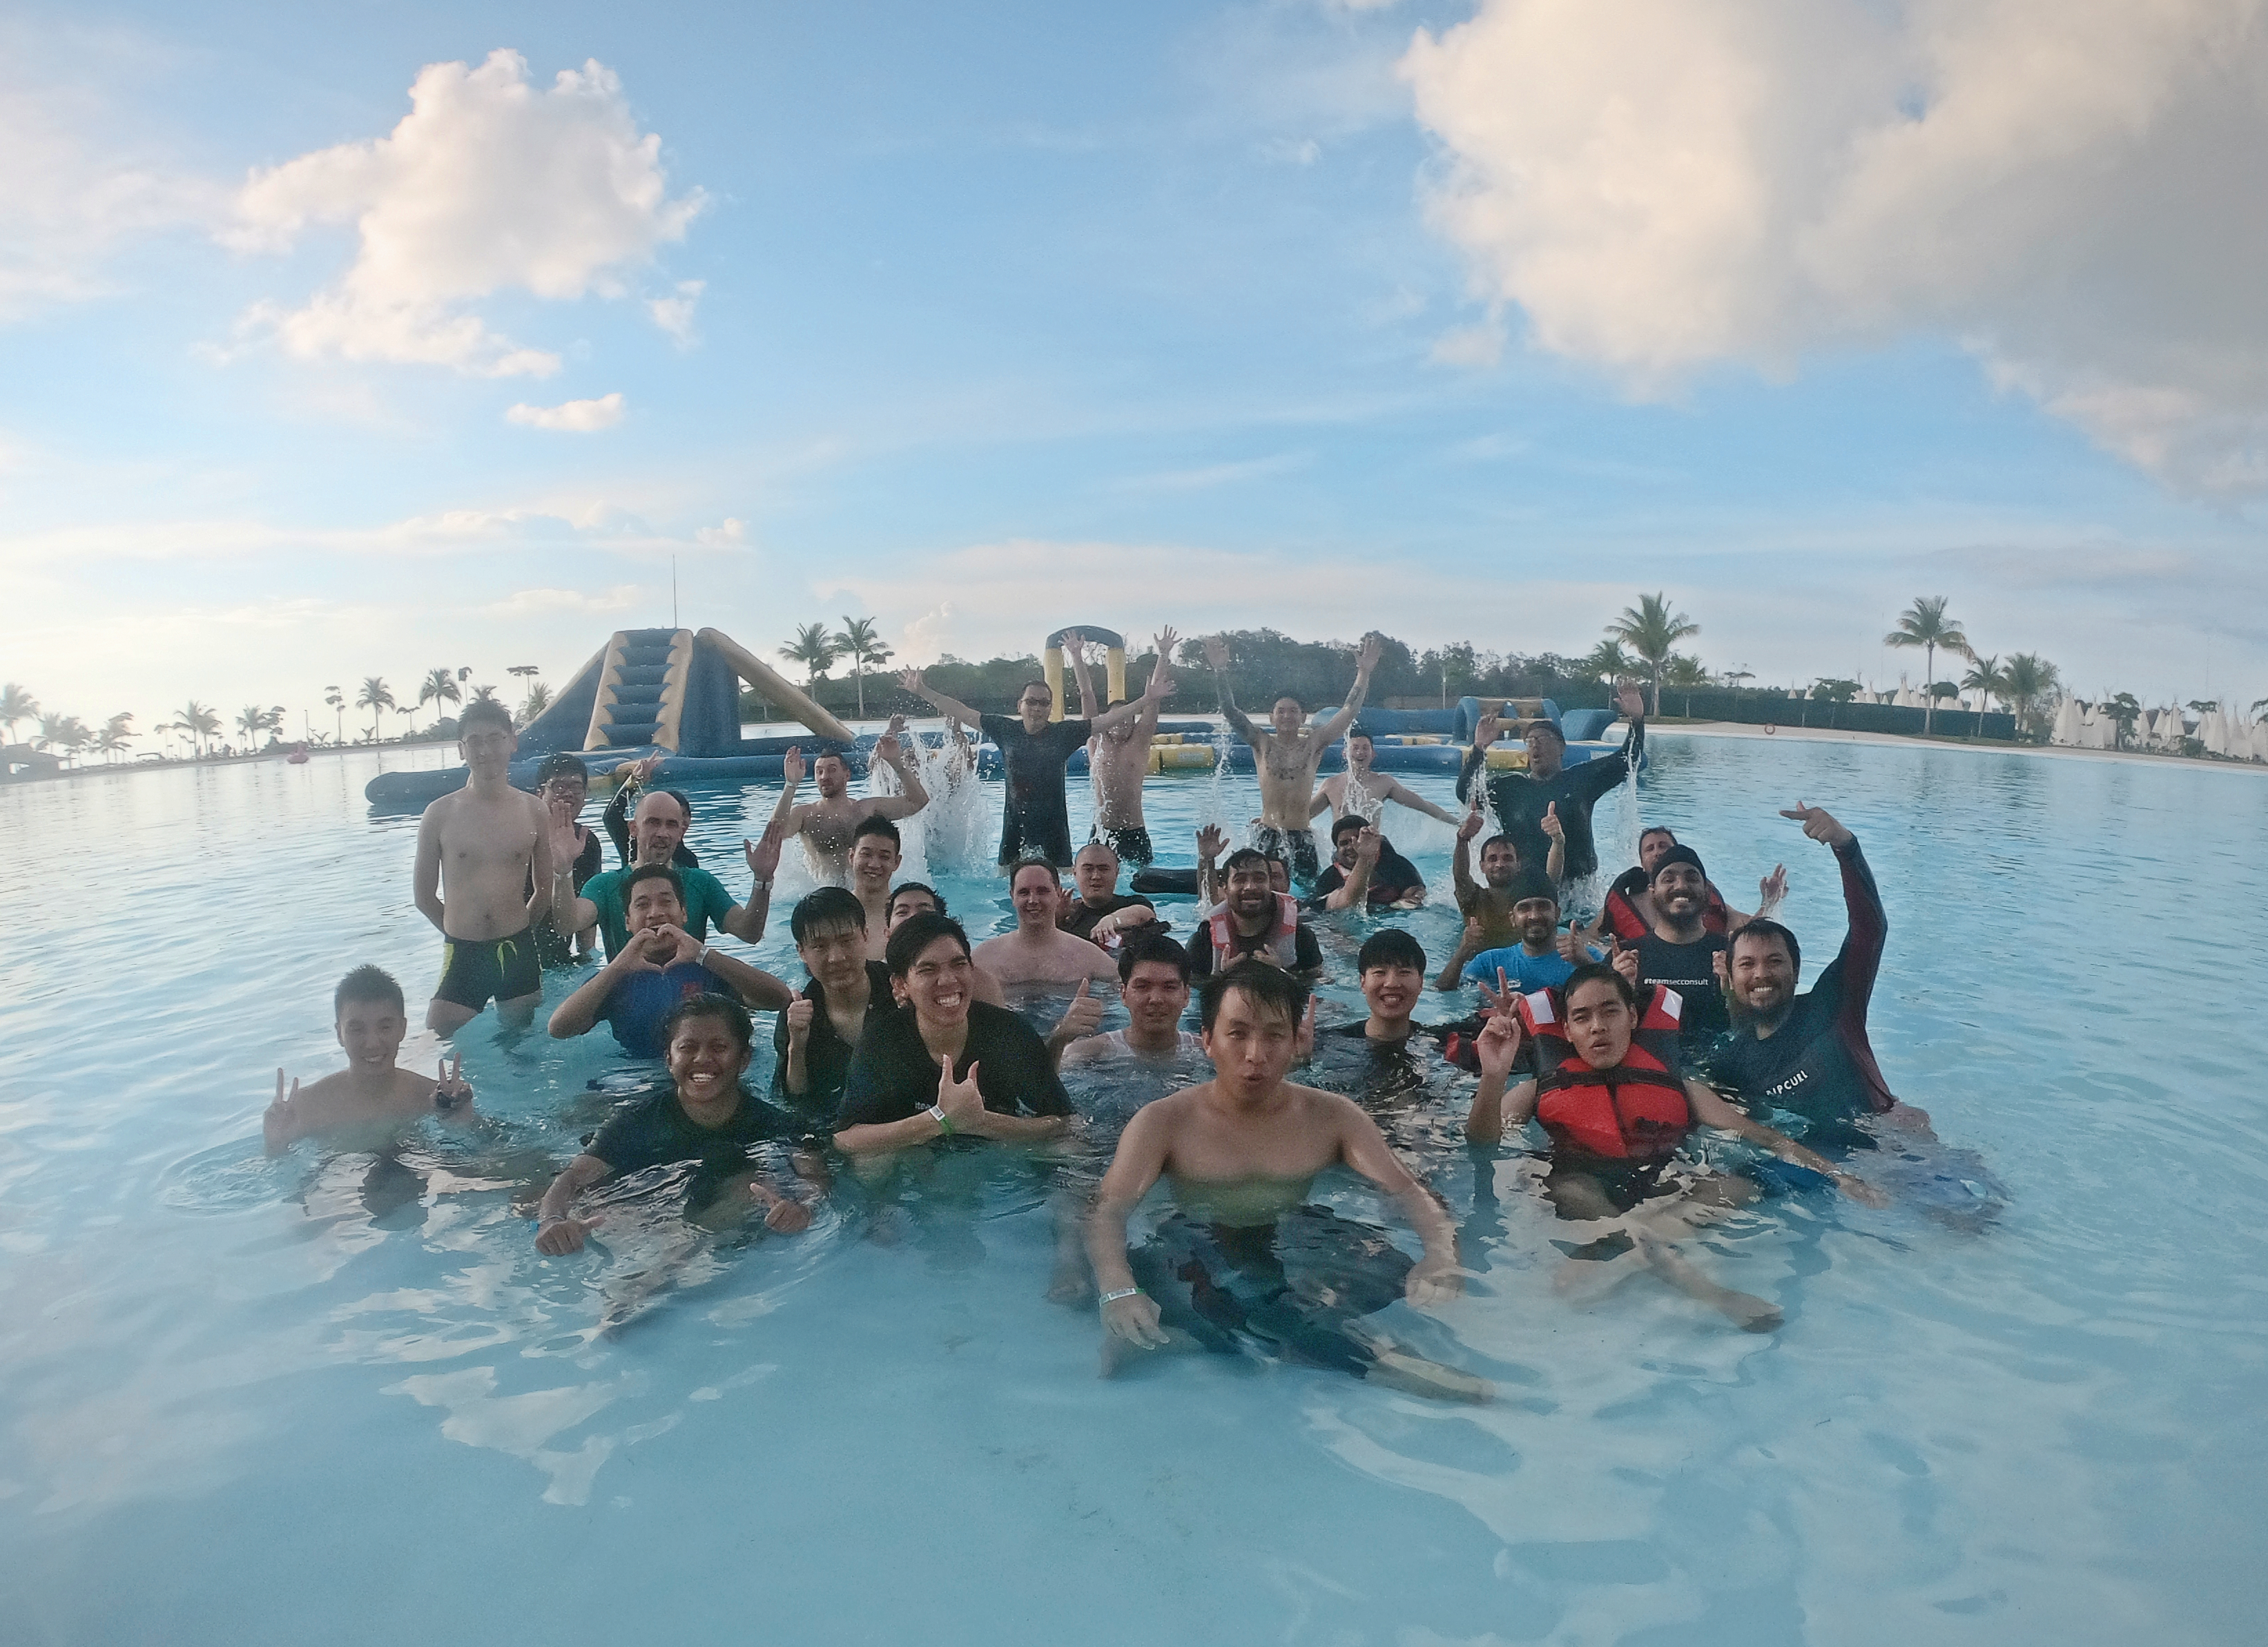
\includegraphics[width=0.45\linewidth]{watersport.jpg}
	}
	\caption{ภาพกิจกรรม Team Event}
	\label{Fig:teamevent}
\end{figure}

\chapter{ประวัติผู้เขียน}

\begin{flushleft}
% ไปใส่รูปในโปรแกรมแก้ PDF
\begin{tabular}{l l}
	\textbf{ชื่อ - นามสกุล} & \AuName \\
	\textbf{Email} & weeruhputt.s@gmail.com \\
	\textbf{ประวัติและผลงานเพิ่มเติม} & linkedin.com/in/weeruhputt \\
\end{tabular}

\end{flushleft}

    
\end{document}